\chapter{Real-time 3D HDR video for EyeTap based on FPGAs and GPUs}
\label{realtimehdrfpgas}

This chapter presents the implementation of a real-time High Dynamic Range (HDR) video 
processing framework in the context of a seeing aid designed for task-specific use (e.g., electric arc 
welding). It can also be built into regular eyeglasses to help people see better in their everyday lives.

The prototype described in this chapter consists of an EyeTap Digital Eye Glass welding helmet and 
a wearable or mobile computer on which a set of image processing algorithms are implemented to 
enable real-time HDR image processing together with applications such as augmented 
reality~\cite{feiner1997touring,starner1997augmented}, mediated reality~\cite{mann1994mediated}, 
and aug-mediated reality~\cite{mannaaai361}. 

The FPGA-based HDR video system runs in real-time and processes 120 frames per second, in 
groups of three frames or four frames (e.g., a set of four differently exposed images captured every 
thirtieth of a second). The processing method, for implementation on Field Programmable Gate 
Arrays (FPGAs), achieves real-time performance for creating HDR video using our novel compositing 
methods, and runs on a miniature self-contained, battery-operated, head-worn circuit board, without 
the need for a host computer.  The result is essentially a stand-alone, miniaturized hardware HDR 
camera system that could be built into smaller eyeglass frames for use in various wearable 
computing and mediated/ aug-mediated reality applications, as well as to help people see better in 
their everyday lives.

Secondly, a highly parallelizable and computationally efficient HDR image compositing, 
reconstruction, and spatio-tonal mapping algorithm for processing HDR video for GPUs is presented 
in this chapter. The algorithms described in this chapter can run on commodity hardware, CPUs and 
GPUs, with the EyeTap Digital Eye Glass electronic seeing aid, and is designed for use in our 
everyday lives. By utilizing the GPU architecture, this approach can be widely adopted for research 
and create customized ``prescription" for various use cases, such as different dynamic range setting 
or different sensor architecture. To validate the robustness of the algorithms, the system was tested 
in extreme dynamic range situations, such as electric arc welding, or looking directly into the sun. 
The GPU-based system also runs in real-time, and requires no user intervention, or fine-tuning of 
parameters after a one-time calibration, even under a wide variety of very difficult lighting conditions 
(e.g., electric arc welding, including detailed inspection of the arc, weld puddle, and shielding gas in 
tungsten inert gas [TIG] welding). The approach can render video with a resolution of 1920x1080 
pixels at interactive and sustainable frame rates of 60 frames per second with GPU acceleration.


The work presented in this chapter was peer reviewed and published in the following list of 
conferences: 

\begin{itemize}
\item
Raymond Chun Hing Lo, Steve Mann, Jason Huang, Valmiki Rampersad, and Tao Ai. High dynamic 
range (HDR) video image processing for digital glass. In Proceedings of the 20th ACM international 
conference on Multimedia, pages 1477�1480. ACM, 2012.
\cite{lo2012high}
\item
S. Mann, R. Lo, J. Huang, V. Rampersad, and R. Janzen. HDRchitecture: Real-time stereoscopic 
HDR imaging for extreme dynamic range. In ACM SIGGRAPH 2012 Emerging Technologies, page 
11. ACM, 2012
\cite{mann2012hdrchitecture}
\item
S. Mann, R.C.H. Lo, K. Ovtcharov, S. Gu, D. Dai, C. Ngan, and T. Ai. Realtime HDR (high dynamic 
range) Video for EyeTap Wearable Computers, FPGA-based Seeing Aids, and Electric Eyeglasses. 
image, 1(2):3�4, 2012.
\cite{mann2012realtime}
\end{itemize}

\section{Introduction}

Existing cameras can only sense a limited dynamic range at any single given exposure, much less 
than the human eye. One method to overcome this limit is to combine differently exposed images of 
the same subject matter, resulting in a High Dynamic Range or HDR image \cite{mannist, comparam,
  robertson2003estimation, kang2003high}. 
  
The history of HDR digital photography goes back almost two decades, as Robertson et al.\ 
stated\cite{robertson2003estimation}:
\begin{quote}
  ``The first report of digitally combining multiple pictures of the
  same scene to improve dynamic range appears to be
  Mann\cite{mannist}''
\end{quote}

With HDR, it is now possible for cameras to match, or even exceed the dynamic range of the human 
eye by orders of magnitudes. The most common method of compositing multiple Low Dynamic 
Range (LDR) images to form an HDR image is to first estimate the photoquantity\footnote{This 
quantity is often incorrectly called radiance or luminance. It is neither, since the spectral response of 
a camera is not flat (i.e. the quantity is not radiance), nor the same as the human eye (i.e. the 
quantity is not luminance).}  by independently transforming each of the input images to an estimate of 
the photoquantity, and then combining these estimates using a weighted sum over a certainty 
function~\cite{mannist, mannwyckofftr, comparam, intelligentimageprocessing}.
This estimate may then (optionally) be transformed via a spatio-tonal mapping (``spatio-tonal 
mappings'' are mappings that depend neither on space or tone alone) for viewing on an LDR display 
(8 bits per channel).  More complex methods relying on per-pixel non-linear optimization are difficult 
to apply directly in a real-time context~\cite{pal2004probability, kang2003high, granados2010optimal} 
as they do not perform linearly and do not have a deterministic runtime.

This chapter presents a real-time wearable HDR seeing aid designed for task specific use 
(specifically, electric arc welding). The prototype EyeTap welding helmet is shown in 
Fig.~\ref{fig:mannvis}, and is known in the welding community as the ``MannVis'' (Mann Vision) 
system.
\begin{figure}[t]
  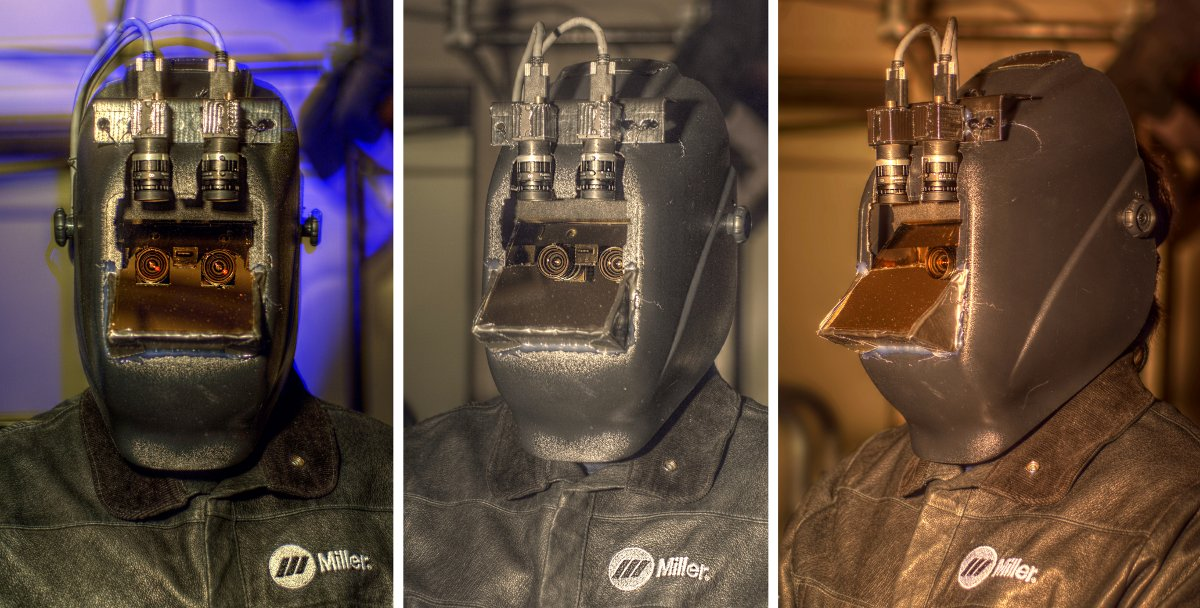
\includegraphics[width=15cm]{ch3/diagrams/cyborg_welding_helmet_2011_02_18_09_53_54_39004100_lowres.jpg}
 \caption{The ``MannVis welding helmet'' implements the EyeTap
   principle which causes each eye to, in effect, function as if the
   eye itself were both a camera and display.  Rays of eyeward-bound
   light are diverted into a pair of downward-pointing cameras by way
   of a diverter, formed from a gold film deposited on the front of a
   welding shade, mounted at a 45-degree angle in the helmet.  The
   shade slides into a slot built into the helmet, so that it can be
   easily replaced if it becomes damaged from splatter, slag, or
   sparks.  The images from the camera are processed for display to an
   audience on a 3D TV, or a live WeldCast$^{TM}$, as well as in the
   wearer's own eyes, where the image is redrawn on the wearer's
   retinas with computer-controlled laser light sources that trace an
   LDR (Low Dynamic Range) image comfortably displaying the more than
   100 million-to-one input dynamic range as a typical 1000:1 output
   dynamic range.  {\bf Note the way in which it appears that the
     wearer has ``glass eyes''.  What we are seeing is a reflection of
     the cameras in the exact position of the wearer's eyes.}  }
 \label{fig:mannvis}
\end{figure}

The real-time video HDR framework, however, has many more far-reaching
applications:
\begin{itemize}
\item as a general-purpose seeing aid, it consists of an EyeTap camera
  system connected to a wearable computer utilizing a set of image
  processing algorithms that improve the wearer's vision through HDR,
  along with mediated and aug-mediated reality;
\item as a drop-in replacement for security cameras, e.g., for general
  purpose surveillance and sousveillance (e.g., inverse surveillance)~\cite{mann2002sousveillance};
\item for general-purpose video cameras both hand-held and
  tripod-mounted.
\end{itemize}

The hardware implementation uses Field Programmable Gate Arrays (FPGAs).  The initial prototype 
includes a low-power (battery-powered) circuit board, which is small enough to fit inside a large
shirt pocket or inside the MannVis welding helmet.

The design is miniaturizable, in the sense that a new circuit board layout can be made to fit into the 
temple side-pieces of eyeglass frames.  The circuit board includes two HDMI camera inputs, one 
being used for the left eye, and the other for the right eye, as well as HDMI outputs fed back to the 
left and right eyes
(head-up displays, EyeTap, or the like), after processing of the video signals.  The current 
implementation runs on a Xilinx Spartan 6, LX45 FPGA, but can be easily adapted to any of a wide 
variety of other FPGAs.

This chapter also presents the state-of-the-art implementation of HDR video processing for extreme 
dynamic range conditions where the scene is relatively static but with high contrast. Unlike previous 
approaches where images are captured with very fine bracketing (e.g., capturing 9 images which are 
one exposure value apart), a scene with a bright light source and dark background (i.e., extreme in 
contrast) is chosen and is captured at 60 fps with 3 different exposures, 4 stops apart. 

%two more examples here
Recently, Michael et al.~\cite{HDRVideoCamera11} proposed a system which captures HDR video 
with an optical arrangement having multiple sensors. One advantage of such a system is its ability to 
simultaneously capture differently exposed images and thus eliminates mis-registration artifacts due 
to motion. Alternatively, modern digital cameras such as the Canon 5D Mark II camera can be 
programmed to capture videos with alternating exposures with a simple modification to the firmware 
(See \textbf{Appendix~\ref{apx:5dIII}}). However, these systems record the videos on flash memory 
and the HDR processing tasks (combining the differently exposed videos and tone mapping) are 
time-consuming offline post-processing tasks that do not run in real-time.  Therefore, such a system 
cannot be used as a real-time seeing aid, nor does the videographer receive immediate visual 
feedback on the recorded HDR videos. 

To address these issues, novel hardware-accelerated algorithms for constructing HDR videos from a 
sequence of alternating exposures, were implemented using GPUs for real-time HDR processing. 
The hardware-accelerated results are useful for seeing aids, as well as being able to shoot videos 
while observing the HDR video result in a viewfinder, display monitor, or other similar outputs. Thus, 
a videographer would be able to compose the shot more effectively while being able to render the 
final result in real-time.

Together with our spatial-tonal mapping algorithm, which is based on a GPU implementation of the 
edge-preserving recursive filter in~\cite{GastalOliveira2011DomainTransform}, real-time (see 
Table~\ref{perf_table}) results that are comparable or better than some of the state-of-the-art tone 
mapping algorithms~\cite{reinhard2002photographic,mantiuk2006perceptual,fattal2002gradient} 
were achieved, especially under extreme lighting conditions such as TIG welding 
(Fig.~\ref{fig:welding_results}).

\section{Background}
 
\subsection{Dynamic range}
Let us begin by defining 2 kinds of dynamic range:
\begin{itemize}
 
 \item 
%%% 
       {\bf Transmitient dynamic range} is the
       dynamic range in signal production.
       For example, the dynamic range of a clarinet is the range from
       quietest sound to loudest sound it can make;
 \item 
 
       {\bf Recipient dynamic range} is a sensed or measured dynamic range,
       such as a sensor's dynamic range.
 
\end{itemize}
 
To the extent that what's between these two is representable as a function, one might call the former 
the {\em dynamic domain} of this function, and the latter its {\em dynamic range}.

One's first encounter with dynamic range is more likely to be the latter than the former, i.e., concern 
for dynamic range (especially its specific quantification in decibels or f-stops) is more likely to arise 
from devices such as sound recorders and photographic cameras than from sound and light sources.

In that sense, we care more about the dynamic range of the human eye or a camera, for example, 
than we do about the dynamic range that could exist philosophically in the {\em transmitient} sense 
(e.g. between bright sunlight and the inside of a coffin in an Egyptian tomb deep underground).

Very few people would ask ``how many dB dynamic range is a clarinet?''.  To answer such an ill-
posed question, do we take the ratio of the loudest note to the silence it produces when sitting on a
desk not being played? Or do we go from the quietest sound it can make to the loudest sound it
can make, regardless of musical integrity?  Or do we take the ratio of undistorted quietest note to 
undistorted loudest note?  The dynamic range would depend on how much distortion we can accept, 
so it becomes very
imprecise in terms of definition.

Let us, therefore, define {\em dynamic range} as follows:
\begin{quote}
  Dynamic range is the ratio
    between the largest and smallest non-negative quantity such
    as magnitude, amplitude, or energy, of
    sound, light, or similar phenomena, for 
    which a small incremental difference in the quantity can still be
    sensed (i.e., the range over which changes in the quantity remain
    discernible).
\end{quote}
Compare with the definition provided in~\cite{tei2011}.
 
\subsection{``Dynamage range''}
 
Let us define an additional concept called ``dynamage range'' as follows:
\begin{quote}
  ``Dynamage range'' is the ratio between the largest quantity
    that will not damage a sensor or device or receiver and the
    smallest non-negative quantity for which changes in the quantity
    remain discernible.
\end{quote}

HDR video was made possible by the invention of cameras that can be overexposed without 
permanent damage.  Unlike old vidicon cameras \cite{Vidiconc95:online} for which the dynamic range 
and dynamage range are roughly equal, modern cameras have a much greater dynamage range 
than their dynamic range.

HDR allows us to increase the dynamic range up to being equal to the dynamage range.


 
\subsection{The EyeTap Principle}
 
The experimental seeing aid system (Fig.~\ref{fig:mannvis}) is constructed with the form factor of a 
standard welding helmet shell, but with two computer-controlled video cameras mounted in a 
binocular configuration facing downwards, pointing toward a welding shade mounted at a
$45^{\circ}$ pitch from the coronal plane.  A gold plating on the welding shade directs the light from 
the front of the wearer toward the cameras. 

Additionally, a computer-controlled stereoscopic display system is built into the helmet, which directs 
light into the wearer's eyes. In this way, the system provides Mediated 
Reality~\cite{intelligentimageprocessing}, a proper superset of Augmented Reality. Augmented reality 
is limited in the sense that it simply adds new matter, but in this case what we really wish is a {\em 
diminished reality}, i.e. to reduce the severity of the contrast ratio locally and selectively such that it 
provides the best possible image to the user. 

The point-of-view of the cameras is the point-of-eye (PoE), such that each camera operates as if it 
were the wearer's own eye. The laser light image forms inside the wearer's own retinas, so as to 
show what is present, but with dynamic range compression when needed. This is called the 
``dynamic range management''. With
dynamic range management, any lighting situation presented to the wearer is managed by the 
computer system to keep the overall lighting in certain ranges.  This is beyond auto-darkening 
eyewear that only manages light levels, because now the contrast, in addition to the light levels 
overall, is managed. 

 
\subsection{Comparametric Equations}\label{sec:comparam}
 
Comparametric equations\cite{comparam} and superposimetric equations~\cite{manders_icip2004} 
are mathematical frameworks for understanding pictures or video of differently exposed or differently
illuminated pictures of otherwise identical subject matter.  This conceptual framework captures the 
general essence of linearity and superposition of light, and in particular, photoquantities, irrespective 
of any non-linearities that might be present in a particular camera system.

In this chapter, the situation where sequential frames of videos, $f_i \in \{ f_1, f_2, f_3, \ldots \} $, are 
captured in rapid succession, with varying exposure levels $k_i$, is considered.  These exposure 
levels are controlled by the wearable computer system to extend the dynamic range, resulting in a 
set of differently exposed video
frames, $f_i = f(k_i q(x,y))$.  This set of pictures is used to estimate the true photoquantity, $q(x,y)$ 
(a spatially varying quantimetric measure of light on the image plane defined by coordinates $x$ and 
$y$).  


% XXX maali: there is nothing in this paper or the implementation
% AFAIK that supports dynamic adaptation to a new camera response
% function

% The first step taken by the wearable computing system is a
% self-calibration step of automatically determining the response
% function(s) of whatever camera(s) happen(s) to be plugged into it.
% This is done by way of automatically solving the comparametric
% equations inherent in each particular camera (every camera has
% associated with it a particular response function, and thus a
% particular comparametric equation that requires solution before
% constructing the HDR pipeline).  

% Following our results in \cite{ali2012ICASSP}, we present here an
% FPGA-based implementation of HDR processing, wherein the HDR
% compositing process is effected using pre-computed \textit{lookup
%   tables} (LUTs), and the tonal mapping for LDR display via an HDMI
% interface is also performed onboard in real-time.

%%%%%%%%%%%%%%%%%%%%
% The problem inherent in solving a comparametric equation may be
% transformed into a problem of solving a differential equation.
% This transformation arises quite obviously from the scaling operators
% commonly used in the study of quantum mechanics, and, specifically,
% quantum field theory.
% Let us proceed with an approach one might find
% in many introductory texts on quantum mechanics
% (see, also, the work of Sophus Lie, the inventor of Lie Algebra):

% In quantum field theory we often use a scaling operator $S_k$,
% and wish to derive an explicit expression for this operator.
% First consider an
% infinitesimally small scaling of the function $f$. Let $\epsilon$ be
% a very small number. We have, up to first order in $\epsilon$
% %
%  
% \begin{equation}
% \label{infsc}
% f((1+\epsilon)q) \approx f(q) + \epsilon \, q
% \frac{\partial}{\partial q} f(q).
% \end{equation}
% %
% By repeated application of the infinitesimal scaling of $q$ we can
% scale $q$ by any amount $e^\Lambda$
% \vspace{-.14in}
% \begin{equation}
% e^{\Lambda} q = \lim_{N \rightarrow \infty}
% \left(1+\frac{\Lambda}{N}\right)^N q.
% \end{equation}
% %
% N-time application of Equation~\ref{infsc} with
% $\epsilon=\frac{\Lambda}{N}$ for $N$ large gives
%  
% \begin{equation}
% f(e^{\Lambda} q) = \lim_{N \rightarrow \infty} \, 
%   \left( 1+ \frac{\Lambda}{N} q \frac{\partial}{\partial q} \right) ^N f(q),  \,\, \\
% %&& \mbox{so that as $N \rightarrow \infty $ we get} \\ 
% %f(e^{\Lambda} q) 
% = \exp \left[ \Lambda q \frac{\partial}{\partial q} \right] f(q) .
% \end{equation} 
% %
% Choosing $\Lambda=\log (k)$ we scale $q$ by $k$ and thus define the
% scaling operator $S_k$ as
% %
% \vspace{-.12in}
% \begin{equation}
% S_k=\exp \left[ \log (k) q \frac{\partial}{\partial q} \right].
% \end{equation} 
% %
% The exponential here is defined as the formal series 
% %
%  
% \begin{equation}
% \exp \left[ 
%     \log (k) q \frac{\partial}{\partial q} 
%   \right] 
% = 
% \sum_{n=0}^\infty \, \frac{(\log(k))^n }{n !} 
%      \left( q \frac{\partial}{\partial q} \right)^n.
% \end{equation}
% %
% Each differential operator in this series acts on every term to the
% right of it.  The inverse of the scaling operator is then
%  
% \begin{equation}
%   (S_k)^{-1} = 
%   S_{1/k} = 
%   \exp \left[ -\log (k) q \frac{\partial}{\partial q} \right].
% \end{equation}
% Now given $g(k,f)$ we can write down $f(q)$ formally as
% %
%  
% \begin{equation}
% \label{formaleq}
% f(q) = S_{1/k} g(k,f(q)).
% \end{equation}
% %
% Although this is not a convenient formulation for explicit
% computation of $f(q)$, it opens the possibility for further analysis
% of the general comparametric problem using the machinery of the
% well-known operators arising in quantum field theory.  Since
% (\ref{formaleq}) holds for any value of $k$, we can take $k$ close
% to one i.e. $k=1+\epsilon$ for $\epsilon \approx 0$ and we see that
% %
%  
% \begin{equation}
%   f(q) =\exp \left[ 
%     - \log (1+\epsilon) \, q \frac{\partial}{\partial q}
%   \right] g(1+\epsilon,f).
% \end{equation}
% %
% If we expand this up to first order in $\epsilon$ we find
% %
%  
% \begin{equation}
% f(q) = \left.\left[1- \epsilon \, q \, \frac{\partial}{\partial q}\right] \left[g(1,f) + 
% \epsilon \frac{\partial g(k,f)}{\partial k}\right]\right|_{k=1}.
% \end{equation}
% %
% Using the identity $f=g(1,f)$ we end up with an ordinary differential equation
% %
%  
% \begin{equation}
% \frac{df}{dq}= \left. \frac{1}{q} \, \frac{\partial g(k,f)}{\partial k}\right|_{k=1}.
% \end{equation}
% %
% from which we can obtain $f(q)$.



\section{Real-time HDR Video Processing}
\label{realtime_hdr}

In this section, a novel HDR image composition method, optimized for FPGA hardware 
implementation of electric eyeglasses, is discussed. This method, advancing upon the results 
in~\cite{mannist,robertson2003estimation,ali2012ICASSP}, is specifically designed for direct 
hardware implementation, as opposed to assuming the availability of a multicore CPU or GPU.  
Additionally, the implementation on how this method can be extended
to three or more images in extreme dynamic range cases using simple
binary operators is presented.
 
\subsection{Mathematical Notation}

Let $f$ represent the \textit{camera response
  function} (CRF), where $f$ in a scalar context is a \textit{tonal
  value}, and in a matrix context $f$ is a \textit{tonal image} (e.g.\
a picture from a camera).  A tonal value $f$ to vary
linearly with pixel value is considered but on the unit interval, and given an
$n$-bit pixel value $v$ returned from a physical camera, $f_i =
(v+0.5)/2^n$ is used, where $N$ images, $i\in\{1,\ldots,N\}$, each
image with exposure $k_i$, are captured. The subscript indicates it is the $i$-th in
a \textit{Wyckoff set}\cite{comparam}, i.e.\ a set of images differing
only in exposure, and by convention $k_{i}<k_{i+1} \;\forall\; i<N$.
$f^{-1}$ is used as the mathematical inverse of $f$ if it has only one
argument, and otherwise as a joint estimator\footnote{A ``joint
  estimator'' is used here in the sense that each photoquantity
  estimate depends simultaneously on multiple measurements.} of the
photoquantity $\hat{q}$.

 
\subsection{Direct Lookup method for combining
  exposures} \label{comp_2_lut}
 
For the case of compositing two images with 8-bit color depth per
channel, a 256$\times$256$\times$3 lookup table (LUT) can be derived for each camera.
The LUT needs to be computed only once each time a new camera is plugged
in for the first time.

 
\subsubsection{Constructing the inverse comparametric LUT}

The inverse comparametric lookup table (CLUT) is a composition of a set
of operations for creating HDR images from an alternating exposure
set.  To construct this look-up table, the response
function of the camera along with its certainty function is estimated using the
method described in Section~\ref{sec:comparam}.

An estimate, $\hat{q}$, of the photoquantity is computed from the
pixel (tonal) values $f_1$ and $f_2$.  This can be by a weighted average
with the certainty function $w$ and with the response function $f$ of
the camera.  To speed up the process (for real-time video), this may be
determined using conditional statements in handling the saturated regions:

\begin{equation}\label{joint_est}
\begin{split}
  \hat{q}=&f^{-1}_{\Delta EV}(f_1, f_2) \\
  =&\begin{cases}
    q_{max}&\text{if $f_1 > \beta$}, \\
    q_{min}&\text{if $f_2 < \alpha$ }, \\
    \frac{f^{-1}(f_1) \cdot w(f_1)+f^{-1}(f_2) \cdot w(f_2) \
      / 2^{\Delta EV}}{w(f_1)+w(f_2)}& \text{otherwise},\\
\end{cases}
\end{split}
\end{equation}
where $\beta$ and $\alpha$ are the saturation parameters of the camera
(Typical values are $\beta$ = 250 and $\alpha=5$.)  and $\Delta EV$ is
the exposure difference between $f_1$ and $f_2$, and $q_{max}$ and
$q_{min}$ are the estimated $\hat{q}$ values at the saturation points,
$f^{-1}(\beta)$ and $f^{-1}(\alpha)$, respectively.

In the prototype, the camera is configured to capture images that are
4 stops apart (i.e., one image has an exposure time that is $2^4=16$
times longer or shorter than the other or has the ISO value 16 times larger or smaller than the other).

Once $\hat{q}$ from the image set is estimated, dynamic range compression (tone mapping) is 
applied for visualization on an LDR display.
Empirically, the following function can provide
adequate dynamic range compression and works well for general high
dynamic range scenes.  

\begin{equation}\label{compressor}
 \hat{q}_{c}=c(\hat{q})=
 r\cdot\hat{q}^{1/k}+d	\\
\end{equation}
where $r$, $k$, and $d$ can be used to adjust ``contrast'' and
``brightness'' of the output image (e.g., k=5, d=-1.0, and r=1.8).

\begin{figure}
\center
 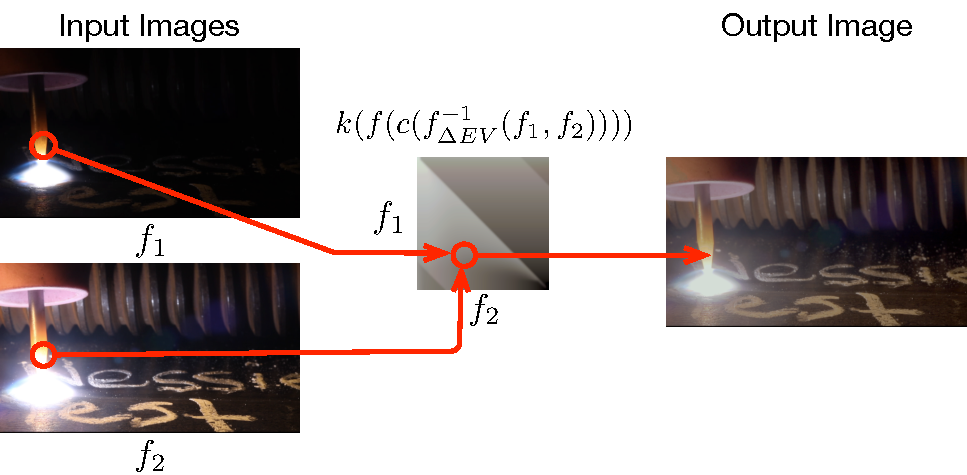
\includegraphics[width=13cm]{ch3/diagrams/direct_lut_method.pdf}
 \caption{\textbf{The composite direct lookup method.} The lookup table $Q_f$ (center) is the value of 
the composition of functions $ k \circ f \circ c \circ f^{-1}_{\Delta EV} $, where  $ f^{-1}_{\Delta EV} $ is 
the joint photoquantity estimator function for two exposures $ {\Delta EV} $ apart, $c$ is the dynamic 
range compression function, $f$ is the CRF, and $k$ is the contrast enhancement function. The value 
of $Q_f (f_1, f_2)$ is evaluated at all possible values of $f_1$ and $f_2$ to create the lookup table 
shown here. This method can be extended to 12-bit or 14-bit images by applying linear interpolation 
to obtain intermediate values from an arbitrarily-sized table.}
 \label{cdlut}
\end{figure}

After a new range-compressed $\hat{q_c}$ is obtained, the output value is estimated by applying the 
CRF to 
$\hat{q_c}$. Since the equation of the CRF may not have a closed form
solution, a nearest neighbor search is applied which
minimizes the absolute distance between $\hat{q_c}$ and $q$
from the response function of the camera.
\begin{equation}
\begin{aligned}
Q = & \underset{z\in \mathbb{N}}{\operatorname{argmin}}{(|f^{-1}(z)-\hat{q_c}|)} \\
\end{aligned}
\label{opt_min}
\end{equation}
Notice that now Q is a quantized output which maps to the range
[0-255] for LDR displays. To further adjust the contrast level of the
image, an additional tonal adjustment function $k$ is applied to
the final result.  
% 
\begin{equation}\label{contrast_enhancement}
 Q_f=k(Q)
\end{equation}
where k can be a simple look-up table for the desired color profile.


% \newcommand{\CDLUT}{\mbox{CDLUT}} 
\newcommand{\CLUT}{\mbox{\textsc{Clut}}}

Lastly, the above function is applied to obtain a solution for all
possible values of $f_1$ and $f_2$. The result
is shown in Fig.~\ref{cdlut}.
\begin{equation}
  \label{combined_function}
  Q_f = k(f(c(f^{-1}_{\Delta EV}(f_1,f_2)))) = \CLUT{}(f_1, f_2)
\end{equation}

\subsection{Compositing 3 or more exposures} \label{comp3_set} 

For the case of constructing HDR images from 3 or more images, an intermediate estimation of the 
photographic quantities
$\hat{q_i}$ is computed using Eq.~\ref{joint_est}. Since the images only differ in
exposures (i.e., 4 stops in our case), the same LUT which precomputed
 $\hat{q_i}$ can be applied to the image pairs at no additional
computational cost.
\begin{equation}
\hat{q_i}=f^{-1}_{\Delta EV}(f_i, f_{i+1}), i \in \{1,..,N\}
\end{equation}
\begin{equation}
\hat{w_i}=\max(w(f_i), w(f_{i+1})), i \in \{1,..,N\}
\end{equation}
Then, the individual photoquantities $\hat{q_i}$ are combined with the
certainty values $w_i$ computed from the last step
\begin{equation}
\hat{q}=g(q_i, q_{i+1}, ... , q_{N-1}, w_i, w_{i+1},...,w_{N-1})
\end{equation}
to create our final estimate of $\hat{q}$.  For the case of 3 images,
the function $g$ can be implemented as a simple weighted average of 
 $q_1$ and $q_2$ with respect to the certainty values $w_1$ and
$w_2$:
 
\begin{equation}
\begin{split}
  \hat{q} = g(\hat{q_1}, \hat{q_2}, w_1, w_2) = \frac{\hat{q_1} \cdot
    w_1 + \hat{q_2} \cdot w_2 / 2^{\Delta EV}}{w_1+w_2}
\end{split}
\end{equation}
One advantage of the proposed algorithm is that the problem is reduced
into sub-steps that can be easily optimized for a specific scenario and
can provide a significant speed-up.

\begin{figure}
\center
  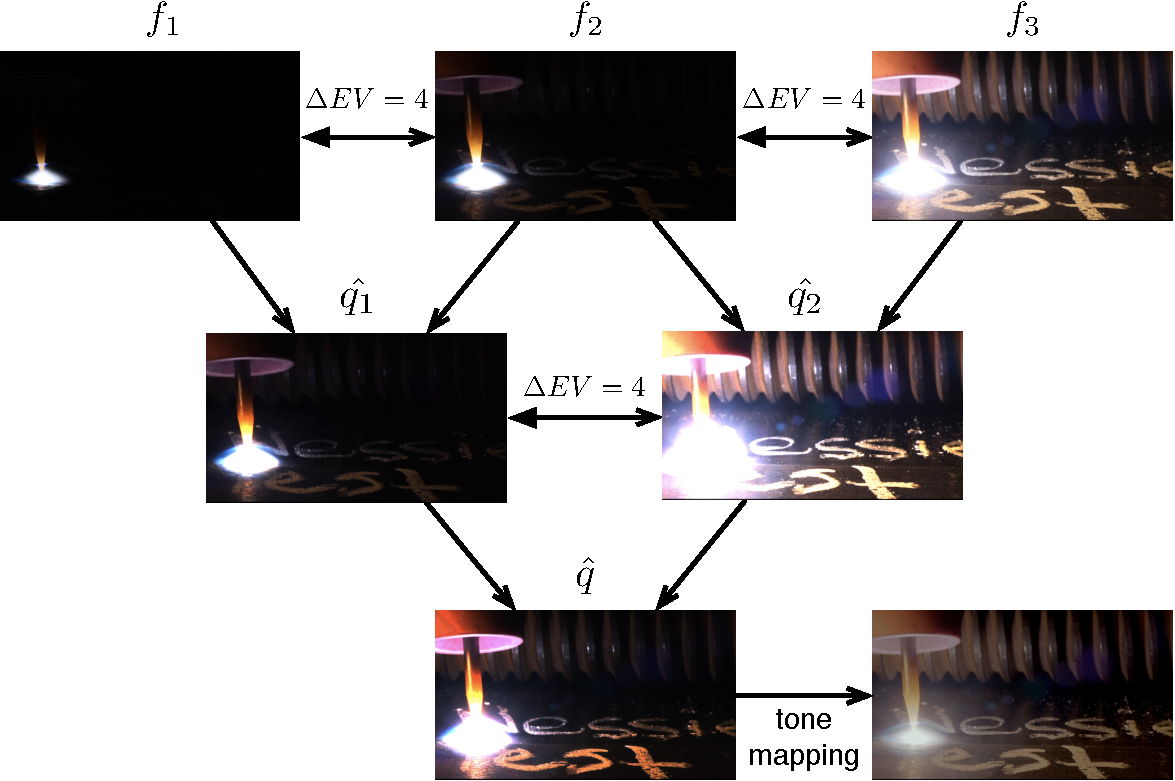
\includegraphics[width=13cm]{ch3/diagrams/3_composite_LUT.pdf}
  \caption{Composition of HDR images using our pairwise approach for
    combining three LDR images, $f_1$, $f_2$, and $f_3$. The final
    estimate of the photoquantity $\hat{q}$ then undergoes
    tonemapping.  }
  \label{composite3}
\end{figure}
With an image set of 3 differently exposed images, the dynamic range is extended by another 4 
stops, a total of 8 stops of additional range.  The compressor function in Eq.~\ref{compressor},
however, is no longer suitable for such a wide dynamic
range. In particular, the contrast of the image was poor and
there was a lack of saturation.  A piecewise function which places
emphasis on the highlights is used.  Despite the simplicity of our
piecewise dynamic range compressor, it provides natural looking
results without accentuating noise and other artifacts: % 
\begin{equation}\label{compressor_new}
  \hat{q_c}=c(\hat{q})=
\begin{cases}
  r\cdot (s \cdot \hat{q})^{1/k}+d& \text{if $\hat{q} \le 1/s$},	\\
  r\cdot (s \cdot \hat{q})^{1/({\gamma \cdot k)}}+d& \text{if $\hat{q}
    > 1/s$}.
\end{cases}
\end{equation}
In the proposed setup, $r=1.8$, $k=4$, $d=-1.2$,
$\gamma=1.5$, $s=140$, and $\hat{q}$ is normalized to [0,1].

Finally, the range-compressed image $\hat{q_c}$ is mapped to the LDR display using 
Eq.~\ref{opt_min} and \ref{contrast_enhancement}. To enhance the local contrast of the final image, 
an unsharp mask is applied to the final image. The final and intermediate results of our algorithm are 
shown in Figure~\ref{composite3}.


\subsection{Exposure pruning for further speedup}
The composition technique introduced in Section~\ref{comp3_set} can be
simplified further by computing multiple LUTs in extreme dynamic range
scenarios.  Under these extreme conditions, e.g., compositing three
images that are 4 stops apart (i.e., $\Delta EV=4$), the exposure
difference between the $f_1$ and $f_3$ is a full 8 stops, ($\Delta
EV=8$).  Since there is very little overlap between lightest and
darkest image, a further speedup can be obtained
by pruning image pairs and discarding the exposures that provide very little or no additional
scene information.  In the case of 3 exposures that are 4 stops apart,
the following conditional statement is used to select the
candidate image pair that would generate our final result using only
LUTs:
\begin{equation}\label{selection_mode}
  Q_f=
  \begin{cases}
    \CLUT(f_2,f_3) & \text{if $f_3 \ge \beta$},         \\
    \CLUT(f_1,f_2) & \text{if $f_1 \ge \alpha$ and $f_3 < \beta$} ,	\\
    0 &\text{otherwise},
  \end{cases}
\end{equation}
where \CLUT{} is the lookup table generated based on
Eq.~\ref{combined_function} with the exposure compensation (i.e.,
multiplying the $\hat{q}$ in Eq.~\ref{joint_est} by $2^{\Delta EV}$)
on $\CLUT(f_1, f_2)$, and $\beta=50$ and $\alpha=20$ are set. Fig.~\ref{3_direct_lut} shows the 
results using this approach.

Furthermore, if the images are also sorted from darkest
to lightest, the two LUTs presented in Eq.~\ref{selection_mode} can be
further compressed into a single LUT with the assumption that the
camera response is monotonic (i.e., $f_1<f_2<f_3$).  Thus, the values
in the upper-triangular (i.e., $f_1>f_2$) part of the LUT can be
replaced by the values from the other LUT.
\begin{figure}
\center
  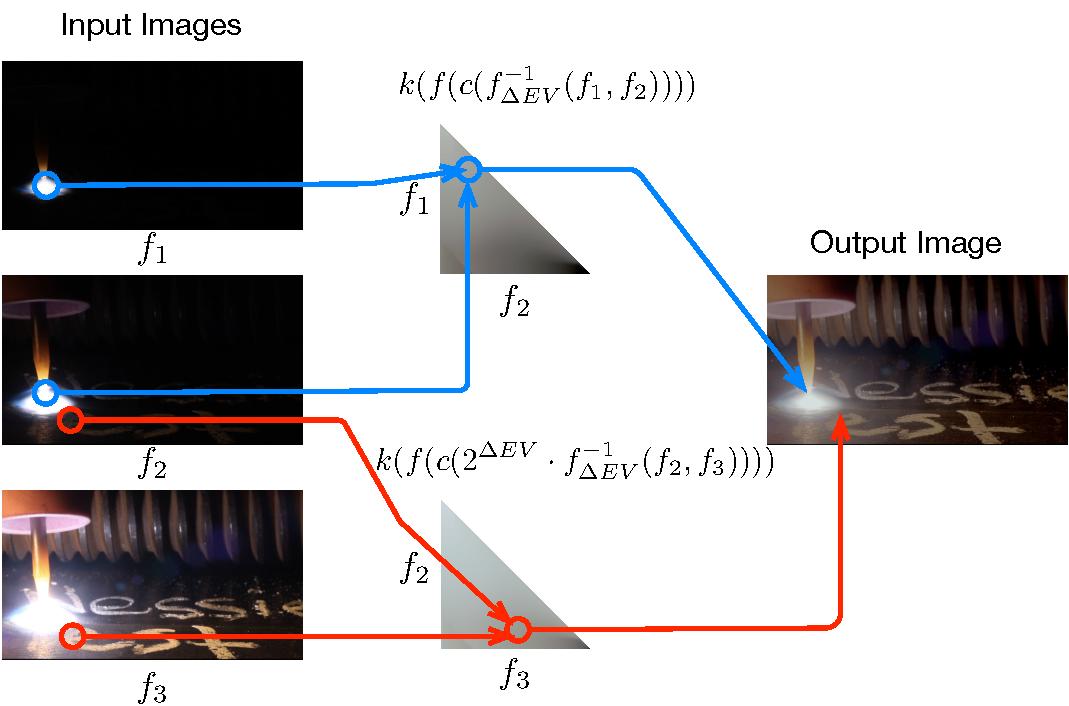
\includegraphics[width=13cm]{ch3/diagrams/3_direct_lut.pdf}
  \caption{Composition of HDR images using a double-LUT approach for
    combining three LDR images, $f_1$, $f_2$, $f_3$.  }
  \label{3_direct_lut}
\end{figure}

% One disadvantage of this approach is that we might see artifacts if
% we applled extreme local contrast enhancement because we are limited
% to 8-bit data.  But the performance and simplicity (i.e. speed up)
% may

%\begin{algorithm}[]
%\SetAlgoLined
%\KwData{N images 8 bits}
%\KwResult{HDR image 8 bits}
%initialization\;
%\While{not at end of this document}{
%read current\;
%\eIf{understand}{
%go to next section\;
%current section becomes this one\;
%}{
%go back to the beginning of current section\;
%}
%}
%\caption{HDR algorithm}
%\end{algorithm}


%discuss the hdr pipeline and our own algorithm for compressing the
% images efficiently over LUTs

%\begin{figure}
%\label{fig:typical_hdr_pipeline}
%\centering
%\includegraphics[width=3.2in]{ch3/siggraph2010_diagrams/data_flow.pdf}
%%\epsfig{file=ch3/siggraph2010_diagrams/HDRchitecture.pdf}
%\caption{A typical HDR video pipeline.}
%\end{figure}



%Figure \ref{fig:typical_hdr_pipeline} shows a typical HDR imaging
% pipeline.  One key contribution of this paper is the use of various
% parallelization and optimization techniques to obtain a real-time,
% interactive, frame rate. For instance, operations such as image
% blending and light space conversion, are highly parallelizable and
% was offloaded to the GPU, thus allowing the CPU to perform other
% operations, such as tone mapping.
%\begin{figure}
%\centering
%
%%\includegraphics[width=1.07in]{ch3/siggraph2010_diagrams/raw_images/weld_picture/
%3_hdr_canon50d.jpg}
%%\includegraphics[width=1.07in]{ch3/ch3/siggraph2010_diagrams/raw_images/weld_picture/
%2_hdr_canon50d.jpg}
%%\includegraphics[width=1.07in]{ch3/siggraph2010_diagrams/raw_images/weld_picture/
%1_hdr_canon50d.jpg}
%%\newline \newline
%%\includegraphics[width=0.8in]{ch3/siggraph2010_diagrams/raw_images/test_80_1038.jpg}
%%\includegraphics[width=0.8in]{ch3/siggraph2010_diagrams/raw_images/test_80_1039.jpg}
%%\includegraphics[width=0.8in]{ch3/siggraph2010_diagrams/raw_images/test_80_1040.jpg}
%%\includegraphics[width=0.8in]{ch3/siggraph2010_diagrams/raw_images/test_80_1041.jpg}
%%\newline \newline
%\includegraphics[height=1.06in]{ch3/siggraph2010_diagrams/raw_images/welding_hd.jpg}
%\includegraphics[height=1.06in]{ch3/siggraph2010_diagrams/raw_images/output0259.png}
%
%\caption{Two instances of the real-time processed HDR images captured
% from our wearable and standalone system by altering the exposures
% between each frame.}
%\label{final_result}
%\end{figure}


%\section{Code Parallelization \\ and Optimization}

%Another key contribution of this work is the use of various optimization techniques to obtain a real-
%time, interactive, frame rate.

%\subsection{GPGPU}
%To obtain an interactive frame rate, the HDR creation process was
% parallelized across the GPUs and the multi-core
% processor\footnote{Nvidia Geforce GTX 460 and Intel
% Core\texttrademark i7-920 Processor}. The HDR video early work by
% Kang \cite{kang2003high} was running at 0.1 frame per second which
% makes the system impractical for real-time usage. Our
% parallelization approach, distributing the tasks across the GPU and
% multi-core processors has provided an interactive frame rate at 25
% frame per second with a single camera setup or with a linear runtime
% tone mapping algorithm \cite{reinhard2002photographic}.
%
%Once we have converted the images to lightspace and recovered the
%radiance map of the scene, the high dynamic photos needed to be
%compressed into a LDR display (usually 8 bits) for viewing. There are
%several tone mapping algorithms we have implemented
%\cite{reinhard2002photographic, mantiuk2006perceptual} .
%
%\begin{figure}
%\label{fig:hdr_pipeline}
%\centering
%\includegraphics[width=3.5in]{ch3/siggraph2010_diagrams/hdr_pipeling_short.pdf}
%%\epsfig{file=ch3/siggraph2010_diagrams/HDRchitecture.pdf}
%\caption{This figure illustrates one of the acceleration schemes used
% in our system. The General Purpose Graphical Processing Unit (GPGPU)
% sequentially creates HDR frames using our precomputed look-up-tables
% and methods proposed in this paper. After a HDR frame is created,
% the main thread passes it to a free tone mapping thread which runs
% on a single CPU. As seen, multiple instances of the tone mapping run
% simultaneously. This pipeline configuration was chosen because: 1)
% the HDR creation is a per pixel operation, which makes it
% parallelizable on the GPGPU. 2) the tone mapping operator involves
% solving optimization problems that may not run efficiently on GPU,
% thus the multiple instances of the the tone mapping are run on the
% CPU instead. A more efficient and parallalizable tone mapping is
% also proposed in this paper to allow for real-time implementation,
% in a trade off for less dramatic tone and detail enhancements.}
%\end{figure}
%
%
%Due to high data dependencies and underlying complexity in the tone
% mapping algorithm \cite{mantiuk2006perceptual}, the tone mapping
% algorithm itself was parallelized at a higher level using pipeline
% technique. Each instance of the tone mapping algorithm was run on
% each CPU core, which provides us 8 instances of the tone mapping
% algorithm. Therefore, as shown in Figure \ref{fig:hdr_pipeline},
% while the GPU creates 8 HDR frames, the CPU is tone mapping the
% previous HDR frames.
%\end{document}  % This is where a 'short' article might terminate


\section{Real-time FPGA-based HDR Video}
%the ability to be portable and battery operated becomes important. 

In order for real-time HDR processing to be practical as a wearable device, a 45nm
low-power Spartan-6 LX45 FPGA
device\footnote{http://www.xilinx.com/products/silicon-devices/fpga/spartan-6/lx.htm}
was selected for its low power consumption and portability.  The board
contains two input HDMI ports used for receiving the baseband HD video
(720p@60fps) and two output HDMI ports used for transmitting the
processed HDR video frames. It also contains 128MB of DDR2 SDRAM
(Micron MT47H64M16-25E, 16-bit data width), used for storing video
frames. It runs at 625MHz in order to meet the real-time processing
requirements. Additionally, BlockRam (BRAM) is used as line buffers
and to store the LUTs. However, it is limited to a capacity of 2.1Mbits
(116 x 18,432).  Due to resource constraints for wearable applications, a focus on reducing
complexity guided us to invent novel approaches to HDR video processing.  Much of
the processing is pre-computed and stored in LUTs to
reduce complexity using the methods discussed in
Section~\ref{realtime_hdr}.  Each pixel sample contains an 8-bit RGB
colour component totalling 24 bits per pixel.  Each lookup table is
addressed by a color channel of two differently exposed frames.  A
total of 16 bits is used for addressing into the LUT totalling
65536 entries.  For an 8-bit wide sample output, the BRAM was configured
as 8-bit wide x 2048-deep which resulted in 32 BRAMs utilized per
color channel for a total of 96 (out of 116) BRAMs utilized.

Efficient on-chip memory utilization is the key to the LUT implementation
technique, as it directly limits scalability beyond 2 frames. The
number of BRAMs required can be reduced by utilizing the fact that
only half of the data in one square LUT is valid, since each pair of
frames has one's pixels always greater than the other's. This
technique is used in 3-frame implementation using the LUTs as
described in Section 3.4.

\begin{figure}
\center
\centering{
  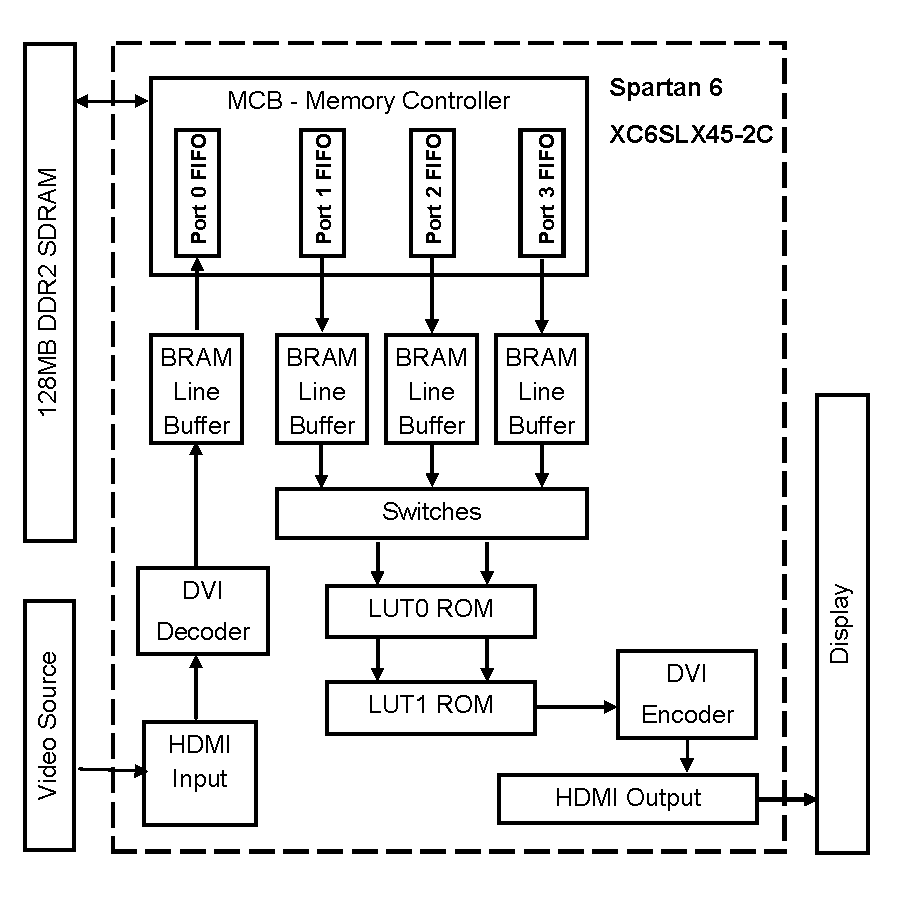
\includegraphics[width=13cm]{ch3/diagrams/hdr_fpga_vertical.pdf}
 }
 \caption { Block diagram of the real-time HDR video implementation
   using a Spartan-6 LX45 FPGA.  Data is received over HDMI and stored
   in line memory.  The frames are stored in external memory and
   concurrently read back line-by-line.  A direct lookup is performed
   on incoming pixel data and the result is sent through an HDMI
   transmitter. }
 \label{fig:fpgahdr}
\end{figure}

A variety of different cameras are used in the prototypes, some with
Firewire interface, some with USB interface, and some with HDMI
interfaces, streaming video through two separate HDMI input ports
(e.g. one camera for left eye, another camera for right eye).  Camera
firmware is often custom programmed so that three or four
differently exposed images of the same subject matter can be acquired in rapid
succession, in the order of weak, medium, and strong exposures.  The
output of each camera is fed to one of the HDMI inputs, as shown in
Fig.~\ref{fig:fpgahdr}.


\subsection{Input Path}
Four Block RAMs (4x8x2048) are used as double-buffered
line memory to hold the decoded video data.  The true-dual ported
nature of the Block RAM allows us to decouple between input video and
memory data path as well as handle the required clock domain crossing
between pixel and memory clocks.  For every horizontal sync pulse
received, the line memory page address is toggled.  The memory
interface runs at 625 MHz and user path utilizes a slightly higher
clock rate (78.125 MHz) compared to the input pixel clock (74.25 MHz)
such that it can guarantee video line storage into memory within a
horizontal sync period.  

\subsection{Memory Interface}
The memory user interface (MIG) guide and CoreGen tool
provided by Xilinx are used to generate a memory controller with data
and command FIFO interfaces. The controller is configured to have six
32-bit data ports, of which one for input data path and three for
readback of the differently exposed images. Request from each port is
serviced by an arbiter in a round robin fashion. Of the 32 bits in the data
width, 24 bits are used to store a pixel. To ensure there is no data loss,
the command FIFO (4-deep) and read FIFO (64-deep) must not overflow
while the amount of data in the write FIFO (64-deep) must be equal to
or greater than the burst length to avoid underflow. Data writes are
executed in bursts of 64 x 4 bytes while reads are executed in bursts of 32 x
4 bytes. The read-back path exposes the pipelined design to parallelism
by fetching all three frames concurrently. The video frame memory
utilizes a circular buffer. As each frame is stored, frame addresses
are incremented at vertical sync.  Because each port will contain both
a light and dark image, a frame multiplexer is used at the input of
the LUT.


\subsection{Output Path}
Three memory ports are used to concurrently read three
lines from each differently exposed frame into the line memory. The
input raster information (h-sync and v-sync) is generated from the input
data and is used to synchronize between all memory read and write
ports. The output of the line memory is fed into a lookup table. The
dual-ported nature of the BRAM allows us to re-use the same ROM for
two lookups. The input of the LUT is multiplexed to correctly feed the
bright and dark frames to the lookup. The output of the lookup table
is then forwarded to a DVI encoder used for transmitting HDMI video.

\section{HDR Compositing for GPU Architecture}

In this section, a generalized HDR image composition method, which is optimized for GPU hardware 
implementation of electric eyeglasses \cite{mannist,robertson2003estimation,ali2012ICASSP}, is 
introduced. Then, an approach to create a real-time HDR video with our pairwise HDR composition 
and spatial tonal mapping method based on the edge-aware recursive filter 
(RF)~\cite{GastalOliveira2011DomainTransform} is presented. The spatial tonal mapping method is 
designed to address the contrast and dynamic range management issues, which the FPGA solution 
may not be able to provide in real-time due to the computation constraints at the moment. The GPU 
approach generalizes the pipeline in multiple stages such as tone mapping which can be individually 
optimized in hardware in the future. The spatial tonal mapping method selected in the proposed 
algorithm is designed for real-time application, and thus it ensures the pipeline runs in a fixed 
processing time. This is critical for the design because any latency induced to the Digital Eye Glass 
inevitably creates user discomfort, which is often worsened with variable latency over time without 
latency management~\cite{jacobs1997managing}. However, latency management is beyond the 
scope of this chapter, and the focus of the chapter is to ensure the latency in the HDR processing 
pipeline is below the display rendering and refresh time, thus providing real-time output to the user 
without any frame drops.

The proposed algorithm in this chapter can run in real-time (30 fps or higher on commodity graphics 
hardware such as the NVIDIA 460 GTX graphics card at 1280x720 resolution) and requires no user 
intervention in the HDR creation process.  The source code of the GPU implementation is listed in 
\textbf{Appendix~\ref{apx:gpu}} for reference. 

\subsection{Direct Lookup method for combining exposures} \label{comp_2_lut}
For the case of compositing two images with three-color (RGB) channels, one inverse comparametric 
lookup table (iCLUT) can be derived for each channel for a specific camera sensor. Each entry of an 
inverse comparametric lookup table results a joint-estimated photometric quantity, $\hat{q}$, from a 
pair of images captured with different exposures. Each iCLUT is composed of $256\times256$ 
entries of 8-bit outputs. The iCLUTs need only be calibrated once for every camera.

Each entry of an iCLUT is estimated by the following equation: 
\begin{equation}\label{joint_est}
\begin{split}
  \hat{q}=&f^{-1}_{\Delta EV}(f_1, f_2) \\
  =&\frac{f^{-1}(f_1) \cdot w_1(f_1)+f^{-1}(f_2) \cdot w_2(f_2) \
      / 2^{\Delta EV}}{w_1(f_1)+w_2(f_2)}\\
%\end{cases}
\end{split}
\end{equation} 
where $f_1$ and $f_2$ are the pixel values from a pair images under different exposure settings; $
\Delta EV$ is the exposure difference between $f_1$ and $f_2$; $f^{-1}$ is the inverse camera 
response and $w$ is the certainty function, proposed by Mann\cite{mannist}.
%The camera response function (CRF) f can be determined using the method described by Manders 
%and Mann \cite{mannist}.
%To construct this look-up-table, we first estimate the response function of the camera along with its 
%certainty function \cite{mannist}.
%An estimate, $\hat{q}$, of the photoquantity is computed from the pixel (tonal) values $f_1$ and 
%$f_2$. 
%This can be estimated by the weighted average of the $f_1$ and $f_2$ with respect to their 
%certainty functions $w_i$ and the response function $f$ of the camera.

%\begin{algorithm}
%\begin{algorithmic}
%\Procedure{RF}{$I$}
%	\State $\left[\frac{dH}{dx}, \frac{dH}{dy}\right] \gets Calculate\_Gradient(I)$
%	\State $Transpose\_Image(I)$ \Comment{Rows become columns}
%	\State $RF\_Y\left(I, \frac{dH}{dx}\right)$            \Comment{To process the rows}
%	\State $Transpose\_Image(I)$ \Comment{Revert to original image}
%	\State $RF\_Y\left(I, \frac{dH}{dy}\right)$            \Comment{To process the columns}
%\EndProcedure
%\end{algorithmic}
%\caption{Computation of a single entry in an iCLUT}
%\label{RF_pseudo}
%\end{algorithm}


\subsection{HDR Composition for 3 or more Images} \label{comp3_set} 
Similar to the FPGA implementation, the composition of the images is performed based on the lookup 
table method. One advantage of using the GPU architecture is that the look up tables and many of 
the operator parameters such as contrast, level of details, color saturation, and HDR mapping range 
for different LDR displays can be tuned at runtime, which allows for full dynamic range control and 
different sensor architecture setup. 

For the case of constructing HDR images from N images (for N $\ge$ 3), the $log(N)$ levels of 
pairwise estimate of the photometric quantities, $\hat{q}_{h,i}$, read as the $ith$ pairwise estimate of 
photometric quantity at level $h$, is computed. At the top level, $\hat{q}_{log(N),i}$ using iCLUT 
generated by Eq.~\ref{joint_est} is computed. For each of proceeding level, its corresponding set of $
\hat{q}_{h,i}$ is estimated by: 
\begin{equation}
\hat{q}_{h,i}=\frac{\hat{q}_{h-1,j}\hat{w}_{h-1,j}+\hat{q}_{h-1,j+1}\hat{w}_{h-1,j+1}/ 2^{\Delta EV}}
{\hat{w}_{h-1,j}+\hat{w}_{h-1,j+1}}
\end{equation}
where
\begin{equation}
\hat{w}_{h,i}=\max(\hat{w}_{h-1,j},\hat{w}_{h-1,j+1})
\end{equation}


%\begin{equation}
%\hat{q_i}=f^{-1}_{\Delta EV}(f_i, f_{i+1}), i \in \{1,..,N\}
%\end{equation}

%Then, we combine the individual photoquantity $\hat{q_i}$ with the
%certainty values $\hat{w_i}$ computed from last step with:
%\begin{equation}
%\hat{q}=g(\hat{q_i}, \hat{q}_{i+1}, ... , \hat{q}_{N-1}, \hat{w_i}, \hat{w_{i+1}},...,\hat{w_{N-1}})
%\end{equation}
%to create our final estimate of $\hat{q}$.  For the case of 3 images,
%the function $g$ can be implemented as a simple weighted average of
%the $q_1$ and $q_2$ with respect to the certainty values $\hat{w_1}$ and
%$\hat{w_2}$:
%\vspace{-.1in}
%\begin{equation}
%\begin{split}
%  \hat{q} = g(\hat{q}_1, \hat{q}_2, \hat{w}_1, \hat{w}_2) = \frac{\hat{q}_1 \cdot
%    \hat{w}_1 + \hat{q}_2 \cdot \hat{w}_2 / 2^{\Delta EV}}{\hat{w}_1+\hat{w}_2}
%\end{split}
%\end{equation}


%One advantage of our proposed algorithm is that we have reduced the problem
%into sub-steps that we can easily optimize for specific algorithm, and
%can provide a significant speed up in those cases. 
%\begin{figure}
%  \includegraphics[width=3.5in]{siggraph2010_ch2/diagrams/4_composite_2.pdf}
%  \caption{Composition of HDR images using our pairwise approach for
%    combining four LDR images, $f_1$, $f_2$, $f_3$, and $f_4$. The final
%    estimate of the photoquantity $\hat{q}$ then undergoes our hardware-accelerated tonemapping 
%algorithm.  }
%  \label{composite3}
%\end{figure}

By capturing 4 images with $\Delta EV=4$, the dynamic range of the HDR image spans a total of 20 
stops $(2^{20}=1,048,576)$ approximately a million to one contrast ratio. To display such a wide 
range on the LDR display, the photoquantity $\hat{q}$ will be compressed with a multi-scale spatial-
tonal mapping algorithm.
%
% history here
%

\subsection{Global Histogram Equalization}
With the power/logarithmic compression, $\hat{q_c}$ often clusters in a narrow range of values and 
thus under-utilizing the displayable range (see Fig.~\ref{fig:welding_results}c). To re-distribute $
\hat{q_c}$ to have a uniform occupancy across the possible displayable range, histogram 
equalization (HE) was adopted to recover the global contrast from the HDR image. Since $\hat{q_c}
\epsilon[0,max(\hat{q_c}))$, normalization is required to bound $\hat{q_c}$ in a known range. To 
perform HE, a histogram of the image as well as the cumulative sum of the histogram was 
constructed:
%h($\cdot$) as equalization operator and $\hat{q_h}$ as equalized estimator,
\begin{equation} \label{histogram_regular}
 \hat{q_h}=HE(\hat{q_c})=\frac{cs(\hat{q_c})-cs_{min}}{M-cs_{min}}max(\hat{q_c})\\
\end{equation}
where $M$ denotes the number of pixels in the image and $cs(v)$ is the cumulative sum of $v$ from 
its histogram. It is known that Equation~\ref{histogram_regular} may over-stretch $\hat{q_c}$ at 
spikes in a histogram (e.g. $h_k \gg h_{k+1}$ and $h_k \gg h_{k-1}$). This may yield undesirable 
result since $\hat{q_c}$ is concentrated in a narrow range of values. The outcome of the equalized 
image then compresses the contrast of the brightest and darkest light values and results in an LDR-
like image. To resolve this behaviour, histogram modification proposed by~\cite{lee2012power} was 
applied:
\begin{equation} \label{histogram_regular}
 m_k=\frac{\log(h_kh_{max}10^{-\mu}+1)}{\log(h_{max}^{2}10^{-\mu}+1)}\\ 
\end{equation}
\begin{equation}
 cs(k)=\displaystyle\sum\limits_{i=0}^{k-1}m_k
\end{equation}
where $m_k$ is the modified value of the original value of the histogram at bin k, $h_k$. The choice 
of $\mu$ moderates the change to the histogram. For large $\mu$, the histogram becomes nearly 
uniform, whereas for small $\mu$ $\ll$ 1, the histogram remains approximately unchanged. $\mu$ = 
5 was chosen experimentally which results in a much more uniformly distributed histogram. 
Consequently, it reduces the over-stretching effect of equalization.
\begin{figure*}
\center
\begin{subfigure}[b]{6.0in}
\centering
  %\includegraphics[scale=0.2, width=4.0cm, bb=0 0 800 1100]{frames/5stops/image3.jpg} 
  %\includegraphics[scale=0.2, width=4.0cm, bb=0 0 800 1100]{frames/5stops/image2.jpg}
  %\includegraphics[scale=0.2, width=4.0cm, bb=0 0 800 1100]{frames/5stops/image1.jpg}
  \includegraphics[width=1.95in]{ch2/diagrams/frames/5stops/image3.jpg} 
  \includegraphics[width=1.95in]{ch2/diagrams/frames/5stops/image2.jpg}
  \includegraphics[width=1.95in]{ch2/diagrams/frames/5stops/image1.jpg}
  \caption{Raw frames captured in exposure bracketing mode (-5, 0, +5 $\Delta EV$). }
  \label{fig:image_set_multiple}
\end{subfigure}

\begin{subfigure}[b]{1.5in}
\centering
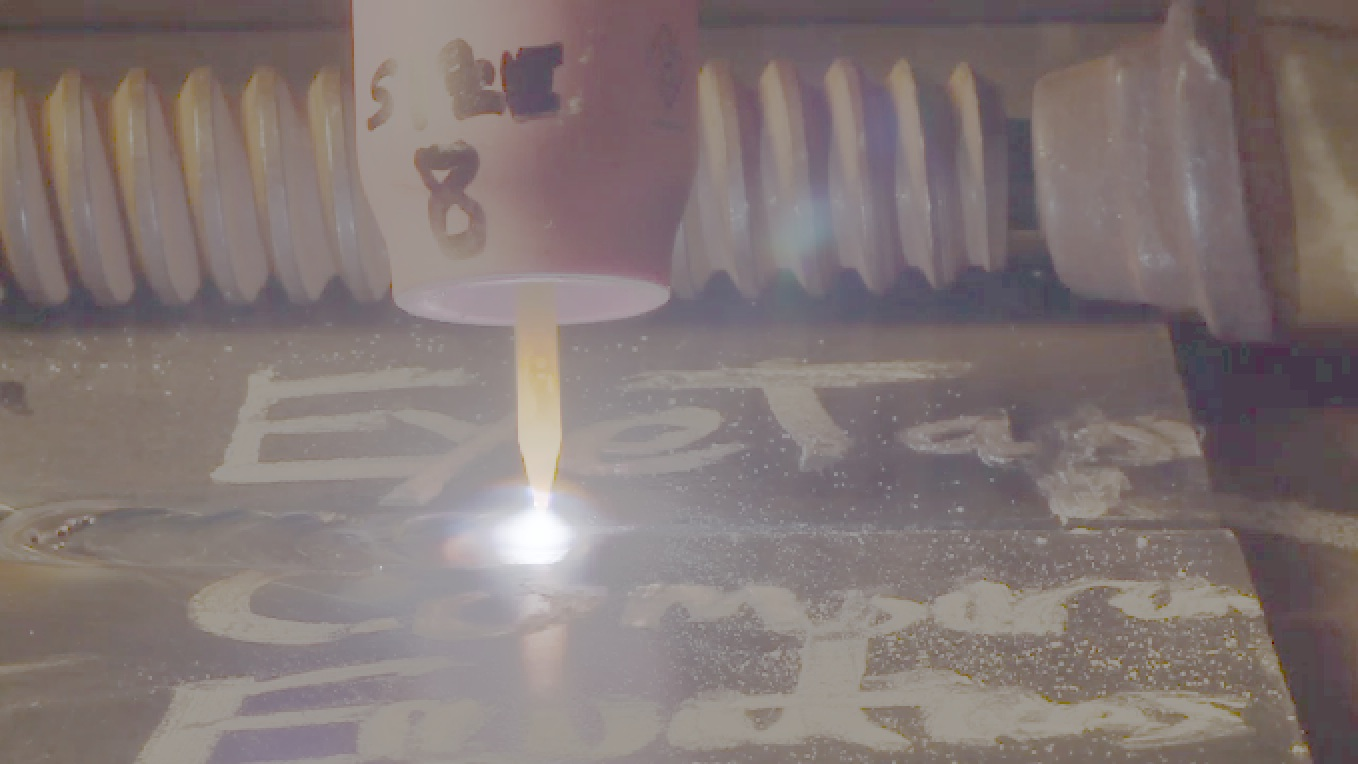
\includegraphics[width=1.4in]{ch2/diagrams/frames/5stops/log_5_stops.jpg}
\caption{Log Compression}
\label{fig:log_compress}
\end{subfigure}
\begin{subfigure}[b]{1.5in}
\centering
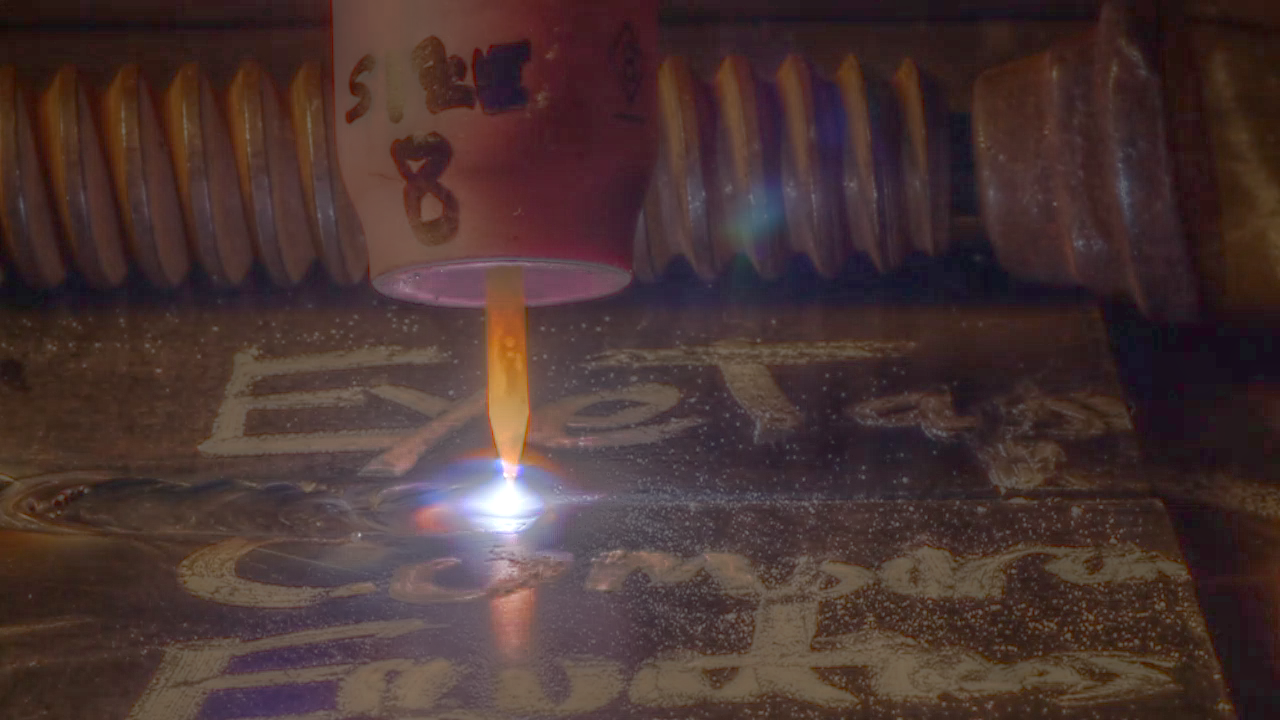
\includegraphics[width=1.4in]{ch2/diagrams/frames/5stops/untitled_pregamma_1_mantiuk06_contrast_mapping_0_1_saturation_factor_0_8_detail_factor_1.jpg}
\caption{Mantiuk, R et al. \cite{mantiuk2006perceptual}}
\label{fig:mantiuk}
\end{subfigure}
\begin{subfigure}[b]{1.5in}
\centering
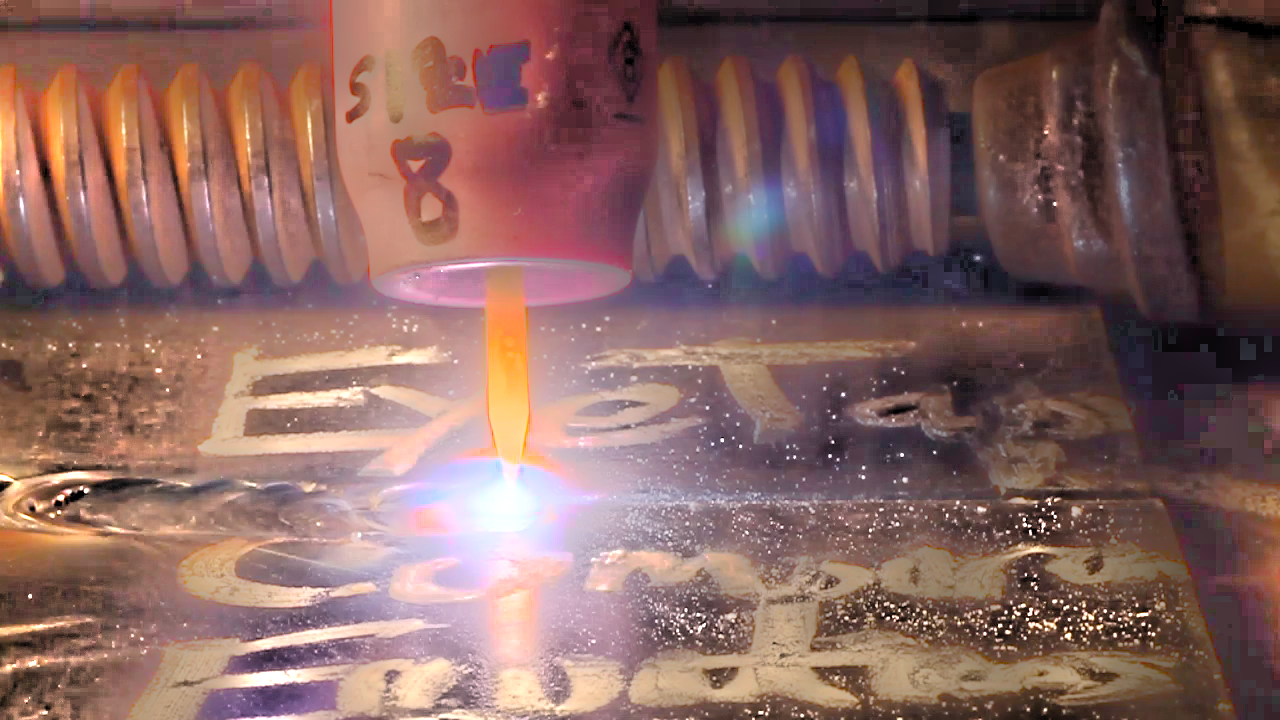
\includegraphics[width=1.4in]{ch2/diagrams/frames/5stops/untitled_pregamma_1_fattal_alpha_0_25_beta_0_57_saturation_0_38_noiseredux_0_fftsolver_1.jpg}
\caption{Fattal, R. et al. \cite{fattal2002gradient}}
\label{fig:mouse}
\end{subfigure}
\begin{subfigure}[b]{1.5in}
\centering
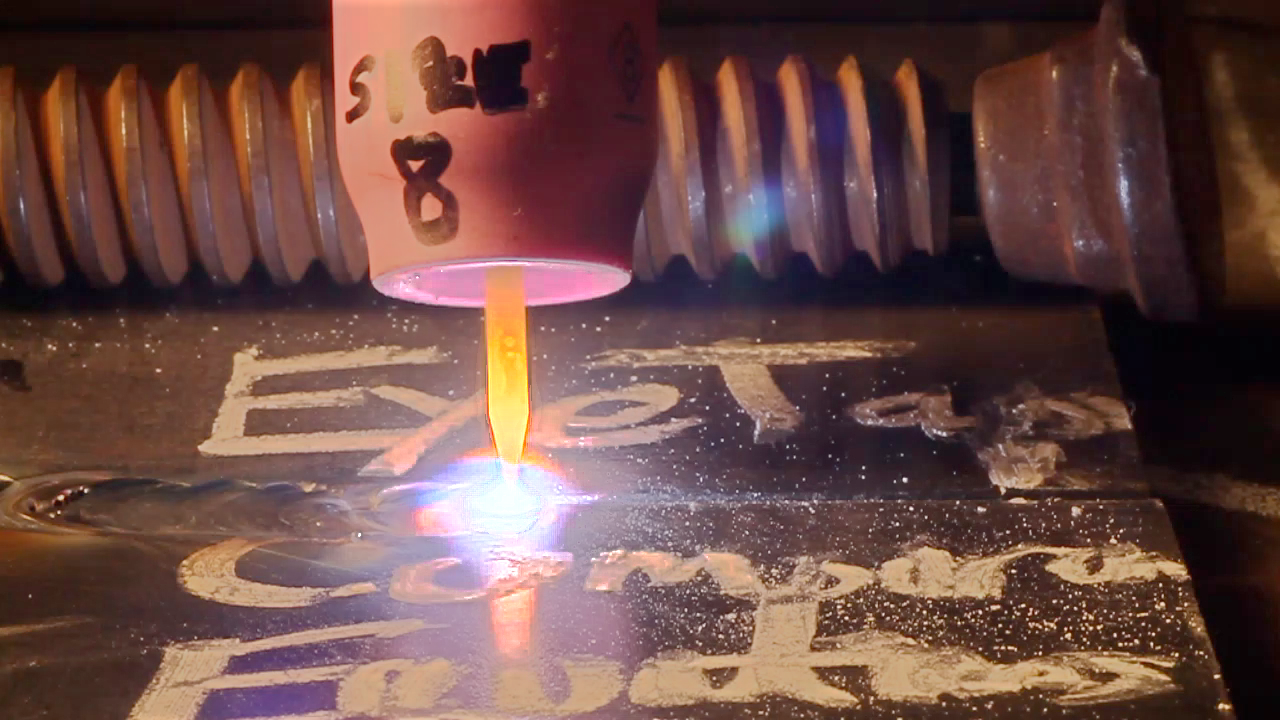
\includegraphics[width=1.4in]{ch2/diagrams/frames/5stops/untitled_pregamma_1_reinhard02_key_0_07_phi_12_2_scales_range_4_lower1_upper90.jpg}
\caption{Reinhard, E. et al. \cite{reinhard2002photographic}}
\label{fig:mouse}
\end{subfigure}        

\begin{subfigure}[b]{6.2in}
\centering
  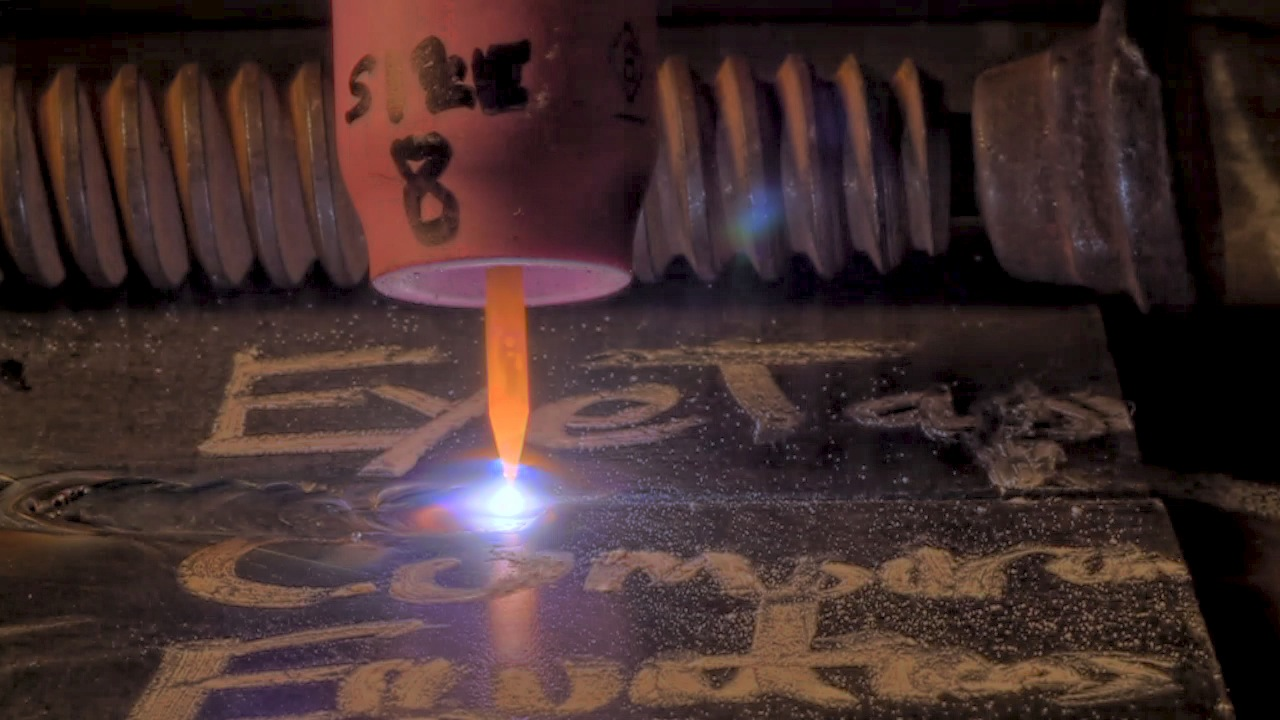
\includegraphics[width=6.0in]{ch2/diagrams/frames/5stops/final_tm_result.jpg}
  \caption{Our result}
  \label{fig:mouse}
\end{subfigure}
%        ~
%        \begin{subfigure}[b]{0.22\textwidth}
%                \centering
%                \includegraphics[width=4.0cm]{frames/welding_set/dark.jpg}
%                \caption{whatever}
%                \label{fig:whatever}
%        \end{subfigure} 
\caption{Results for HDR video of extreme dynamic range.
                 Notice that the tip of the tungsten electrode is only visible
                 in the darkest exposure, and the background is only visible
                 in the lightest exposure.
                 Our result, shown in (f), is the only of the spatio-tonemapping
                 algorithms that can render the very tip of the tungsten
                 electrode and background both clearly.
                 (d-f) Tone mapping results from 
\cite{mantiuk2006perceptual,fattal2002gradient,reinhard2002photographic} using the Luminance 
HDR program.
                 In extreme cases, the HDR composition method by~\cite{debevec2008recovering} 
introduced artifacts in the shadow area, and the tone mapping algorithms further amplified these 
defects in the final images.
                Our result is not only better than these tone mapping algorithms (and the only one to 
faithfully show the tip of the tungsten electrode)
                but it is also capable of running in real-time.}\label{fig:welding_results}
\end{figure*}


\section{Multi-scale Spatial Tonal Mapping}
%halo free, much less artifact than the other two (compare with fatal,etc...)
With a global tonal mapping operator, the HDR results obtained from the previous section appear 
relatively low in contrast and saturation when dealing with extreme dynamic range scenes. To 
improve the visual appearance of the images on an LDR display, the HDR image can be compressed 
based on not only tonal information, but also spatial information such as gradient or edges. Although 
a number of tone mapping algorithms have been proposed, very few tone mapping algorithms have 
been designed for real-time video usage. In particular, the tone mapping algorithms which show high 
quality results often involve non-linear optimization which has a high complexity and is difficult to be 
parallelized due to its non-deterministic runtime. On the other hand, the algorithm reported in 
\cite{reinhard2002photographic}, which has low computational requirements and is easy to be 
parallelized, produces halo artifacts, low contrast, and non-natural looking results. Moreover, some of 
the tone mapping operators are only designed for images and produce temporal artifacts such as 
flickering and color shifting throughout the process.

Recently, a computationally efficient edge-preserving filter \cite{chen2007real, 
GastalOliveira2011DomainTransform} has shown promising results in performing tone mapping on 
HDR images. The recursive filter (RF) ~\cite{GastalOliveira2011DomainTransform} is shown to be 
particularly well-suited for decomposing the image in real-time on graphics hardware.

The proposed approach for real-time tone mapping and composition, which is based on 
\cite{GastalOliveira2011DomainTransform} and \cite{farbman2008edge}, provides the natural looking 
and stable results among a variety of conditions (see Fig.~\ref{fig:welding_results} for comparison).
%The contribution of our work is the design of a complete HDR algorithm that can run on graphics 
%hardware or FPGAs in the future.
%list a few tone mapping algorithms here%
%see figure for the L value.
%see the compressed value
%decomposition
%detail layers
%controls
%
%see the final value
%\subsection{Global Dynamic Range Compressor}
To compress the high dynamic range images, the log luminance, $L_c$, of the image was first 
estimated based on the final estimate of photoquantities on the RGB channels, $\hat{q}_r$, $\hat{q}
_g$, $\hat{q}_b$, from section 2.2.
\begin{equation}
L_c = log(0.2989*\hat{q_r} + 0.5870*\hat{q_g} + 0.1140*\hat{q_b} + 1).
\end{equation}
Then, the dynamic range of the luminance channel is compressed using a logarithmic compressor 
with a simple offset to avoid negatives values.
\begin{equation}
L_c = log(L+1).
\end{equation}
Alternatively, more natural looking images, but with less contrast, can be obtained with the following 
compressor function: 
\begin{equation}\label{lum_equation_2}
L_c = L^{l/\gamma}
\end{equation} where $\gamma \ge 1$ and $c > 0$.

Then, $L_c$ is normalized and compressed to the range $[0,1]$. The range can be adjusted at 
runtime, which has effects on detail extraction, with the $s$ and $d$ parameters (typically set to 
$s=8.0$, $d=5$).
\begin{equation}\label{lum_equation_3}
L = s*L_c+d
\end{equation}
In the proposed setup, a moving average filter on $max_L$ and $min_L$ is applied to avoid flickering 
due to any sudden luminance changes in the scene.

\subsection{Local Contrast Enhancement}
The global tone mapping operation, such as logarithmic compression, from the last step provides us 
a base image which is often lacking contrast. The local contrast (spatial-tonal mapping) can be 
applied with the multi-scale edge-preserving decomposition method. This method is found to be 
effective for compressing HDR images in extreme cases (see the clear rendition of the tip of the 
tungsten electrode with our proposed method in Fig. 1b).
To extract details from the image and enhance their local contrast, the multi-scale edge-preserved 
smoothed images $J_i$ are created where i $\in\{1,..,M\}$ using the recursive filter (RF) discussed in 
\cite{GastalOliveira2011DomainTransform}.
\begin{equation}\label{lum_equation_4}
J_i = RC (L, \sigma_s, \sigma_r, k)
\end{equation}
where $\sigma_s$ and $\sigma_r$ are the filter spatial and range standard deviation, and k is the 
number of iterations the filter smooths the image. In particular, $\sigma_s$ = 20, $\sigma_r$ = 0.0825 
is used for extracting $J_1$; $\sigma_s$ = 50, $\sigma_r$ = 0.165 is used for extracting $J_2$; $
\sigma_s$ = 100, $\sigma_r$ = 0.335 is used for extracting $J_3$ and $k=1$. The detail layers $D_i$ 
are obtained by finding the difference between $J_{i-1}$ and $J_i$, with $J_0=L$, where each 
succession of the detail layer contains coarser details than the previous layer. The detail layers are 
weighted and summed to reduce to a single contrast mask $L_f$ as follows:
\begin{equation}
L_f = 0.9*J_M + \sum_{i=0}^{M-1}{a_i D_i}
\end{equation} where $a_i$ is the desired weight for each layer. In our setup, $a_0=0.4$, $a_1=0.3$, 
$a_2=0.3$ is used which emphasizes the texture from the layer containing the finest details. From 
the observation and experiment, this setting allows greater local contrast of tonal values in the 
extremely bright and dark areas of the scene. To obtain a displayable output image, the photoquantity 
$\hat{q}$ is compressed using the contrast mask in Eq.~\ref{lum_equation_4} and is quantized to the 
standard 24-bit RGB pixel values:
\begin{equation}
\begin{split}
f &= round(255.0*(\hat{q}/10^{L})^{\gamma} \cdot L_f), \\
\end{split}
\end{equation}

%Table~\ref{table:layers}.
%\vspace{-0.5cm}
%\begin{table}[!h]
%\center
%\caption{The parameters for the 3 detail layers used in our system.}\label{table:layers}
%\begin{tabular}{|c|c|c|c|}
%\hline
% & $J_1$ & $J_2$ & $J_3$ \\
%\hline
%$\sigma_s$ & 20.0 & 50.0 & 100.0 \\
%\hline
%$\sigma_r$ & 0.0825 & 0.165 & 0.335 \\
%\hline
%\end{tabular}
%\end{table}

From our experiment, this filter is more computationally efficient than bilateral filter n large kernel 
size. This is a critical requirement for our HDR compression algorithm as the runtime remains 
constant regardless of the parameter settings. Furthermore, it does not introduce temporal artifacts 
(such as flickering) and the result is consistent (e.g., the histogram equalization approach often 
produces inconsistent results under difficult lighting conditions). This is critical in HDR video because 
any incoherence between the adjacent frames can be distracting to the audience.
Once the smoothed edge-preserving images are obtained, the detail layers are extracted by 
subtracting the adjacent images from the stack.
\begin{equation}
D_i = J_i - J_{i+1}
\end{equation} where $J_0=L$, and i $\in \{0,..,K-1\}$.
Then, our final results are composed by first normalizing the $J_N$ channel as our base image with 
the following linear mapping:
\begin{equation}
B = \frac{J_K - min_J}{max_J - min_J}
\end{equation}
where $[min_J, max_J]$ is the desired range mapping to the LDR image (e.g., 24-bit display with 8 
bits per channel) and
%where $max_J$ and $min_J$ are the desire range we would like to mapped to our LDR.
 the parameter $\gamma$ controls the saturation in the final image (typically set to between $0.5$ to 
$0.7$). 


Overall, there are two main advantages of using the edge-preserving filter proposed by 
\cite{GastalOliveira2011DomainTransform}. First, the parameters $\sigma_s$ and $\sigma_r$ 
empower users to refine their emphasis of detail enhancements. Second, the fine tuning of the $
\sigma$ parameters helps to minimize the halo artifacts compared to traditional image decomposition 
based on the Laplacian pyramid. Qualitatively, the output of our HDR rendition is better than many 
other approaches as shown in Fig.~\ref{fig:welding_results} and it can also run at constant time which 
is important for wearable applications.

It is worth noting that this tone mapping algorithm is spatially dependent (i.e., the input resolution and 
the number of layers both have to be considered). For example, with higher-resolution videos, it may 
be necessary to use additional layers (i.e., 4 layers instead of 3 in this case). Fortunately, the 
algorithm proposed is independent of other parameter settings such as brightness, contrast, and 
detail manipulation, since the size of the video is constant. These properties are critical to the design 
of an HDR system used in our daily lives, as the latency of the system has to be predictable. 
Furthermore, the proposed solution shall be scalable to a higher resolution as more capable 
hardware becomes available in the future.

\section{Performance Analysis}
The algorithms described in the previous section are specifically chosen and designed to be 
parallelized on GPUs and can also be implemented on FPGAs in the future.
%To show the feasibility of our approach, the Direct LUT method described in 
Section~\ref{comp_2_lut} were implemented with the 3 alternating frames on FPGAs.
\subsection{GPU performance}
\begin{table}[!h]
\center
\begin{tabular}{|l|r|r|}
\hline
%Tone Mapping Operator  & Time(ms) & Frames Per Second & Speed-up \\
\bf{Tone Mapping Operator} & \bf{FPS} & \bf{Speed-up}\\
\hline
Mantiuk, R. et al. \cite{mantiuk2006perceptual}     & 0.58              & $143.42\times$\\
\hline
Fattal, R. et al. \cite{fattal2002gradient}        & 0.58              & $142.5\times$\\
\hline
Reinhard, E. et al. \cite{reinhard2002photographic}     & 6.49              & $12.83\times$\\
\hline
Implemented Edge-Preserving Method          & 83.33             & $1\times$\\
\hline
\end{tabular}
\caption{This table shows the run-time of different Tone Mapping Operators and the speed-up of 
using our implemented method. Our implementation 
achieves approximately 80 frames-per-second; which is several times faster than other tone mapping 
operators.}
\label{perf_table}
\end{table}

Computation using GPU maximizes acceleration on algorithms that run on a large matrix with 
independent element operations. The proposed HDR algorithm relies heavily on per pixel operation 
without much cross dependencies with neighbour pixels. The runtime cost of each operation in 
milliseconds, benchmarked on a NVIDIA 460GTX, over 150 videos (over 100 minutes of footage) at 
the resolution of 1280x720 are as follows. The operations of pixel-to-photoquantity conversion and 
the compression by logarithm requires on average $1.5ms$. Normalization on images are done using 
efficient min/max finder from the NVIDIA's CUBLAS library, which costs around $0.8ms$ per call. The 
spatial tone mapping is the least parallelizable part of the process, which consumes up to $12ms$. 
The edge-preserving filtering for three layers executed in parallel takes up $11ms$ of runtime, 
becomes the main contributor to the overall latency in the proposed HDR pipeline. This is due under 
utilization of available thread pool of the GPU architecture. Per iteration the RF only requires as many 
threads as the size of one dimension of the image multiplied by the number of color channels. In the 
proposed implementation, we launch the filter on a monotone channel, $L$ which is a gray scale 
representation of the image, to reduce the total amount of computation required. Other optimization 
techniques such as matrix transpose are applied to ensure coalesced memory access patterns. The 
remainder of $1ms$ runtime is contributed by the contrast enhancement stage after obtaining the 
layers using RF. Overall, the HDR composition and tonal range compression algorithm cost $17ms$ 
(~60fps) on average, and that is suitable for real-time system. 

%The general rule in GPU computing is to avoid excessive memory transfer between the machine 
%and graphics card. In our application, since every step can be computed using GPU, the memory 
%transfer is only required upon receiving a new frame. Since the transfer overhead with latency is as 
%low as 1$ms$ per frame per direction (e.g., host to device or device to host), it is relatively 
%insignificant comparing to the latency due to the construction of HDR image. Global memory 
%access on GPU is usually expensive in comparison to shared memory and thread cache. Frequent 
%access to read/write global memories as intermediate update could cause high latency and drop 
%performance of the construction. Another expensive operation is due to thread synchronization 
%after each kernel call. Therefore, 

%\begin{table}[!h]
%\center
%\caption{Average latency per stage of HDR construction for a $1280\times720$ image on a NVIDIA 
%Tesla C2050 with 3 detail layers.}
%\begin{tabular}{|l|c|}
%\hline
%Operation & Time (ms) \\
%\hline
%Light space conversion & 1.5 \\
%\hline
%Local Contrast Enhancement with RF & 24.0 \\
%\hline
%\end{tabular}
%\end{table}


%\subsection{FPGA}
%
%The algorithm which uses direct look up table is implemented on a Spartan-6 LX45 FPGA device 
%for its low power consumption and portability. %(See Fig~\ref{fig:FPGAHDRchitecture}). 
%The supply power measured for the system is 1.448W, thus it allows the application to run for 
%around $20$ hours on a typical rechargeable battery with capacity of $5800$mAh.
%The board contains High Definition Multimedia Interface (HDMI) input ports used to receive video in 
%$720\times480$ at 60 frames per second, and output HDMI ports used to transmit HDR video 
%frames. 
%Two differently exposed video frames of the same subject matter are supplied via the HDMI input in 
%rapid succession, in an alternating order.
%The frames are stored into memory and read out concurrently for composition.
%The 128MB of DDR SDRM (Micron MT47H64M16-25E, 16-bit data width) on the board is 
%configured to run at 625MHz data rate to store video frames.
%The board also contains 2.1Mbits (116x18432bits) Block RAM (BRAM) in total, which are used for 
%line buffers and to store pre-computed LUT results.
%
%The post processing starts by compressing the produced HDR images with a square root.
%Then it converts the color space from RGB to YCrCb, in order to save the resources that needed 
%for implementation. Converted luma channel is convolved with multi-stage a 5-by-5 Gaussian Kernel 
%for extracting two layers of edges from the original HDR image.
%The edges are then scaled and added back to the original image for bringing back the detailed 
%textures.
%
%The 4-up display mode was created to provide a real-time visualization of multiple exposures,  
%  enabling the user to simply point a camera and see the frames that comprise the HDR 
%composition. 
%This allows for easier testing and calibration of the input frames for HDR video processing %(See 
%Fig~\ref{diagram_4up}).
%The maximum latency of the implemented logic is 223ns, whereas the DDR2 memory access used 
%up 80 percent of the processing time.

%\begin{figure}
%\center
% \includegraphics[width=7.5cm]{fpga_images/acmmm12_fpga.pdf}
% \caption{FPGA-based HDR architecture for the 4-up display capabilities.}
% \label{fig:FPGAHDRchitecture}
%\end{figure}

%\subsubsection{Real-time HDR Streaming Using 2 frames}
%Real-time HDR composition of 2 differently exposed frames was implemented using direct look-up 
%tables (LUTs).
%For combining two images~\cite{ccece2012hdrEyetap}, pre-computed 8-bit values are stored into 
%Block RAMs (BRAM).
%In order to implement one LUT, it requires 65556-entries (256 x 256) times 8 bits per entry, which is 
%equivalent of 524kbits. 
%This requires 1.5Mbit (524kbits x 3 channels of RGB) to cover the two images with 8-bit RGB color 
%space.
%Since the Spartain-6 FPGA contains 2.1Mbits of BRAM, a more efficient memory utilization method 
%is required to enable HDR involving more than two frames. 

%\subsubsection{4-up HDR display, enabled by FPGA}
%Push buttons and switches connected to the FPGA are configured such as to enable switching the 
%order of dark, medium, bright frames, and turning on/off 4-up mode. 
%To be included as a hand-held screen for the final prototype for portable real-time HDR device, this 
%4-up screen enables users to calibrate exposures quickly and accurately on the go.  

%In the process of implementing the 4-up display, a constraint was put on the design to ensure that 
%no change was required to the original data path. 
%This requirement was crucial to the overall modular design of our FPGA HDR architecture. 
%This only adds two modifications to the original data path, both of which are controlled via push-
%button switches. The switches allow for easy change to the original data path without the 4-up - 
%useful for when the full-screen or eyeglass-mounted display or EyeTap resolution is desired for just 
%the combined HDR video.

%diagrams for the flow
%fixed aperture (DOF) 
%low ISO (noise)
%only alter the shutter speed

\section{Applications}
The new possibilities of ``seeing'' beyond human eye capability become a fascinating experience, to 
me, and many others who experienced the 3D HDR Digital Eye Glass prototypes the first time. The 
initial reactions from many of the first time users are very positive. Often, users are surprised about 
the additional amount of extra details they can discover around the world. The additional textures, 
colors, and depth cue that the Digital Eye Glass can provide a teleported hyper-reality experience in 
which one can perform many tasks such as welding in the dark that were once prohibited by our own 
senses. 

The spatio-tonal mapping algorithm, which allows for real-time tuning for details extraction, can serve 
as a true seeing aid for improving contrast or even perform color remapping for individuals who may 
have visual related problems such as color blindness. In this section, a set of potential applications 
which derives from enabling 3D HDR are described that can be applied in everyday life.

\subsection{Personal Safety and Driving}
\begin{figure}
\center
 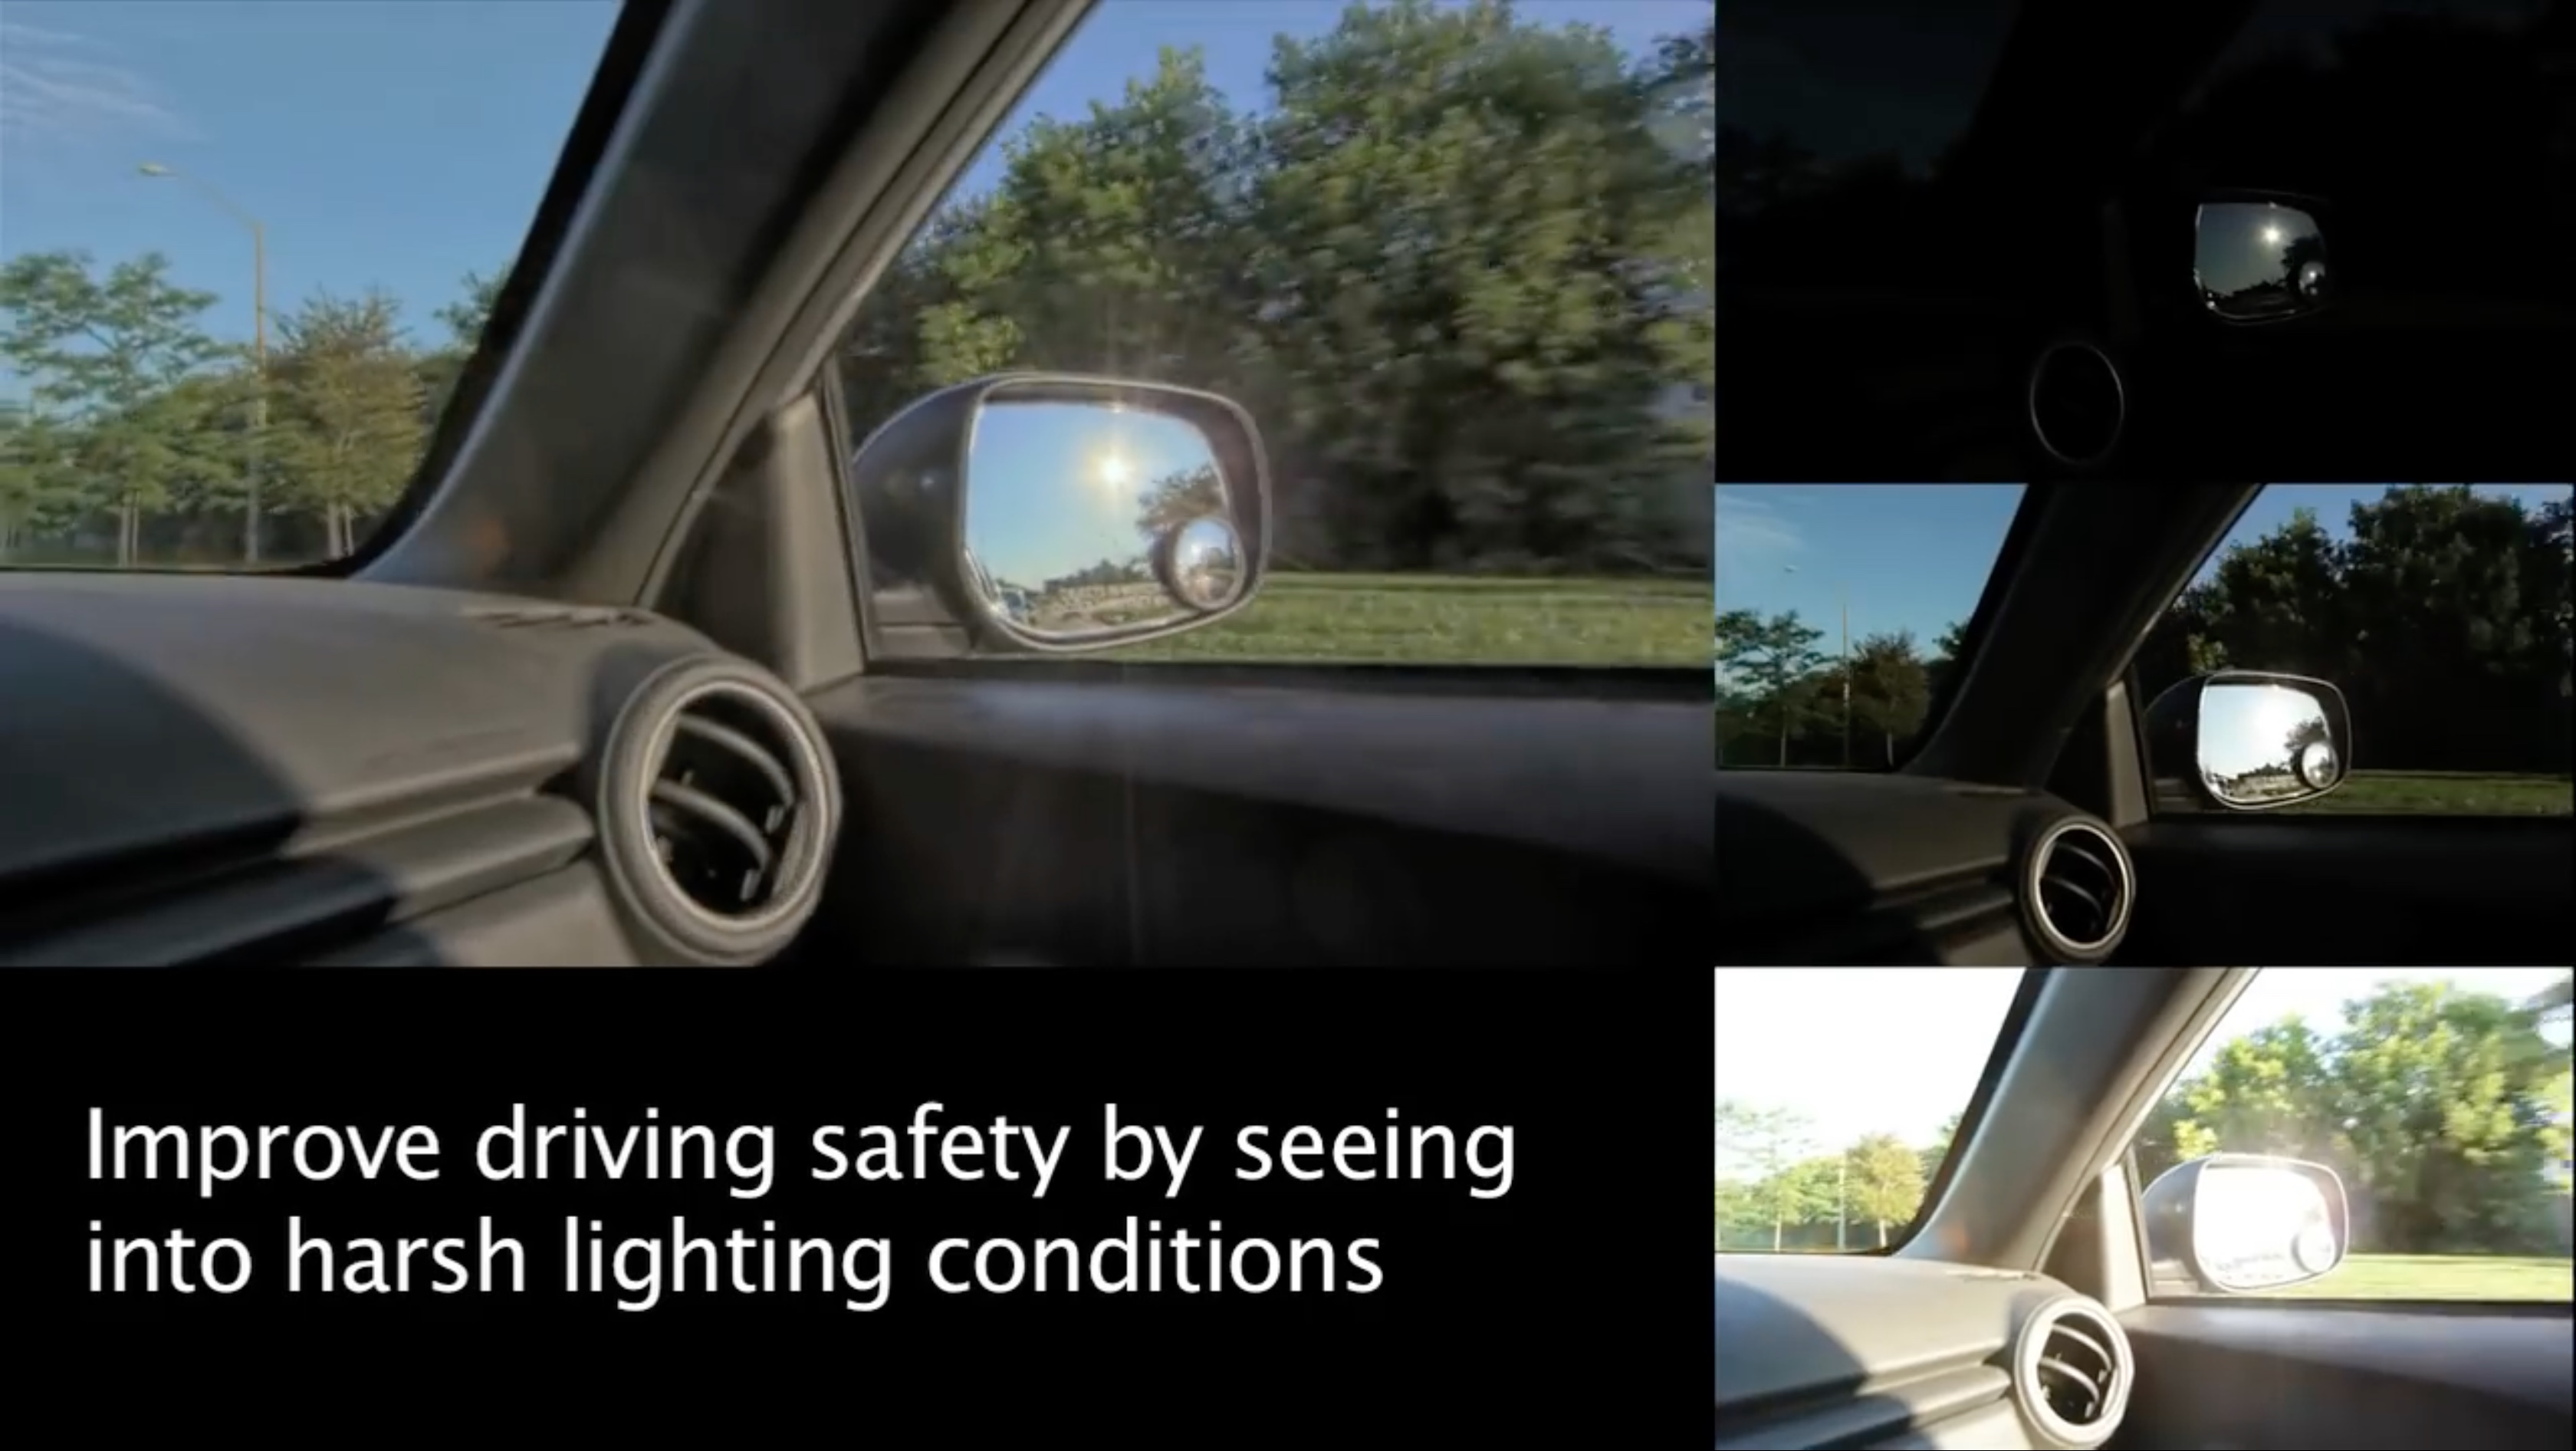
\includegraphics[width=5.5in]{ch2/diagrams/everyday3.jpg}
 \caption{Example of HDR in real life driving situation. 3 different exposures, 4 stops apart, were 
taken, and combined into the HDR images shown on the leftmost. With the HDR video, the sun, and 
the passenger side can both be visible at the same time. More importantly, the sun from the side 
mirror is no longer blinding the driver, and we can now see everything clearly inside and outside of 
the car.}
 \label{fig:extremeeveryday3}
\end{figure}
Dynamic range issues are often more pronounced in everyday life scenes such as driving. Many 
unexpected road conditions, especially the harsh lighting conditions in different time of the day, 
creates many dangerous situation to the driver. Many of us may recall the eye blinding moment from 
exiting a tunnels in bright sunny days or when a car's head light or the sun light hitting directly onto 
our eye.  At those times, the dynamic range of the scene scene is either too dark or too bright for the 
human eye to adapt quickly, and such moments of blindness can often cost a life or death decision. 
Fortunately, the proposed HDR approaches provides a robust way of handling lighting conditions for 
both indoor and outdoor situation. In Fig.~\ref{fig:extremeeveryday3}, a harsh and rather common 
driving condition is shown. The sun is shining directly into the driver's eye and at any given exposure 
it is not possible for the camera to see the side mirror and outside condition clearly.

\begin{figure}
\center
 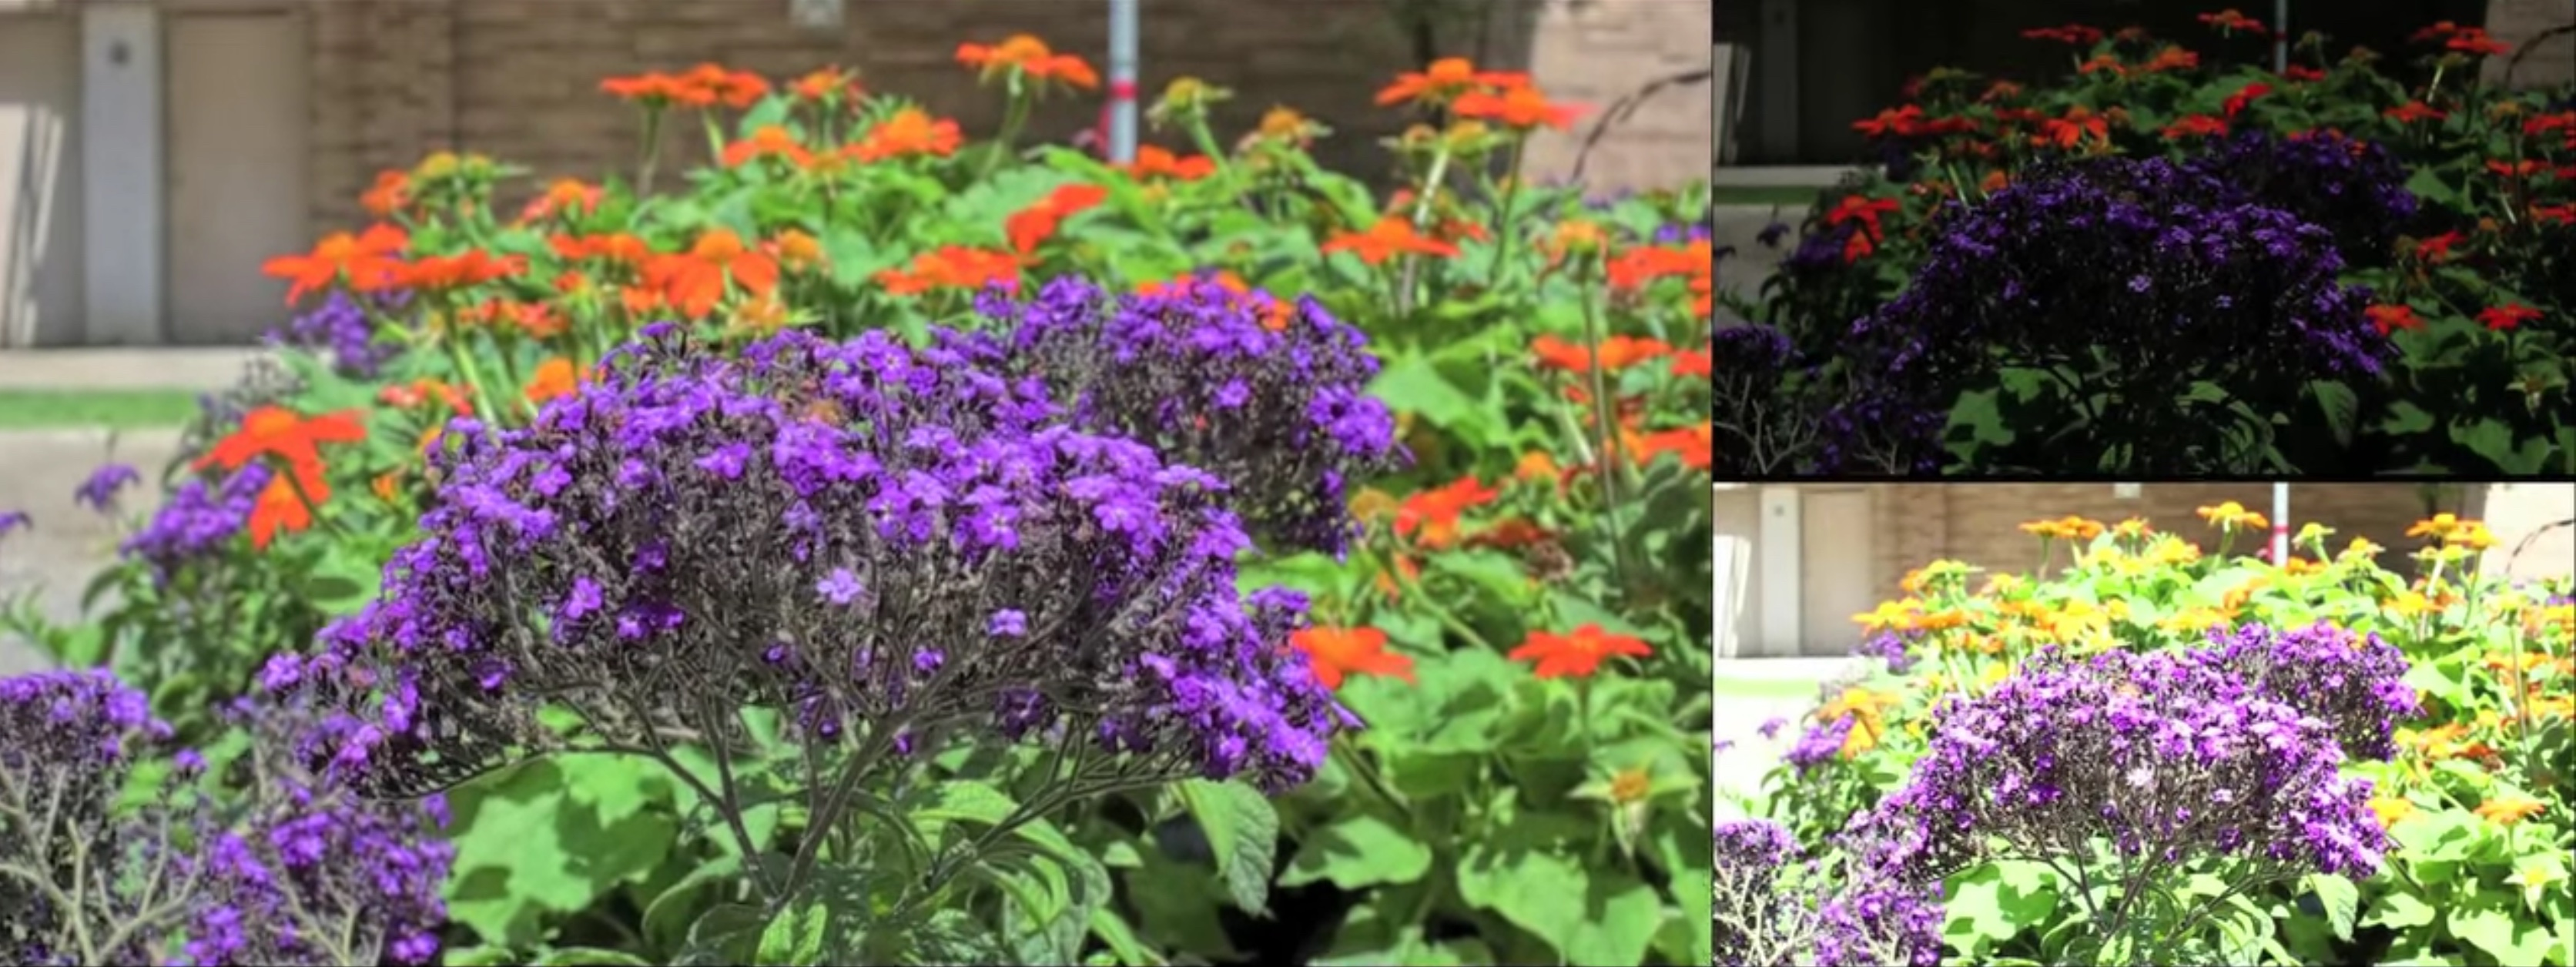
\includegraphics[width=5.5in]{ch2/diagrams/everyday1.jpg}
 \caption{Example of HDR and color enhancement. The HDR can also prevent saturation from each 
channel, and thus can enhance the final color fidelity of the image. The final color can also be 
remapped for color-blinded individual if needed.}
 \label{fig:extremeeveryday1}
\end{figure}

The proposed HDR pipeline also allows for many customization such as color saturation adjustment 
and remapping. In many of the everyday outdoor scene, color can easily be saturated (clipping) in 
one of the channels. With the HDR, the full spectrum is captured and the tone mapper can now 
individually adjust the saturation level per channel. For example, in Fig.~\ref{fig:extremeeveryday1} 
the red channel was clipped in the higher exposure image, while the blue channel was clipped in the 
low exposure image. By combining both exposures, a super color image can be composed and 
remapped such that the saturation per channel can be managed. The super-natural look of the final 
rendering can be adjusted on-the-fly. In Fig.~\ref{fig:extremeeveryday2}, a high contrast scene was 
captured, and shown the potential use of the eyeglasses for day-to-day documentary purposes. 
Despite the strong sun light is reflected from the glass, the multiple exposures approach can capture 
both the highlights as well as shadow detail and remapped naturally back onto a single HDR image.

\begin{figure}
\center
 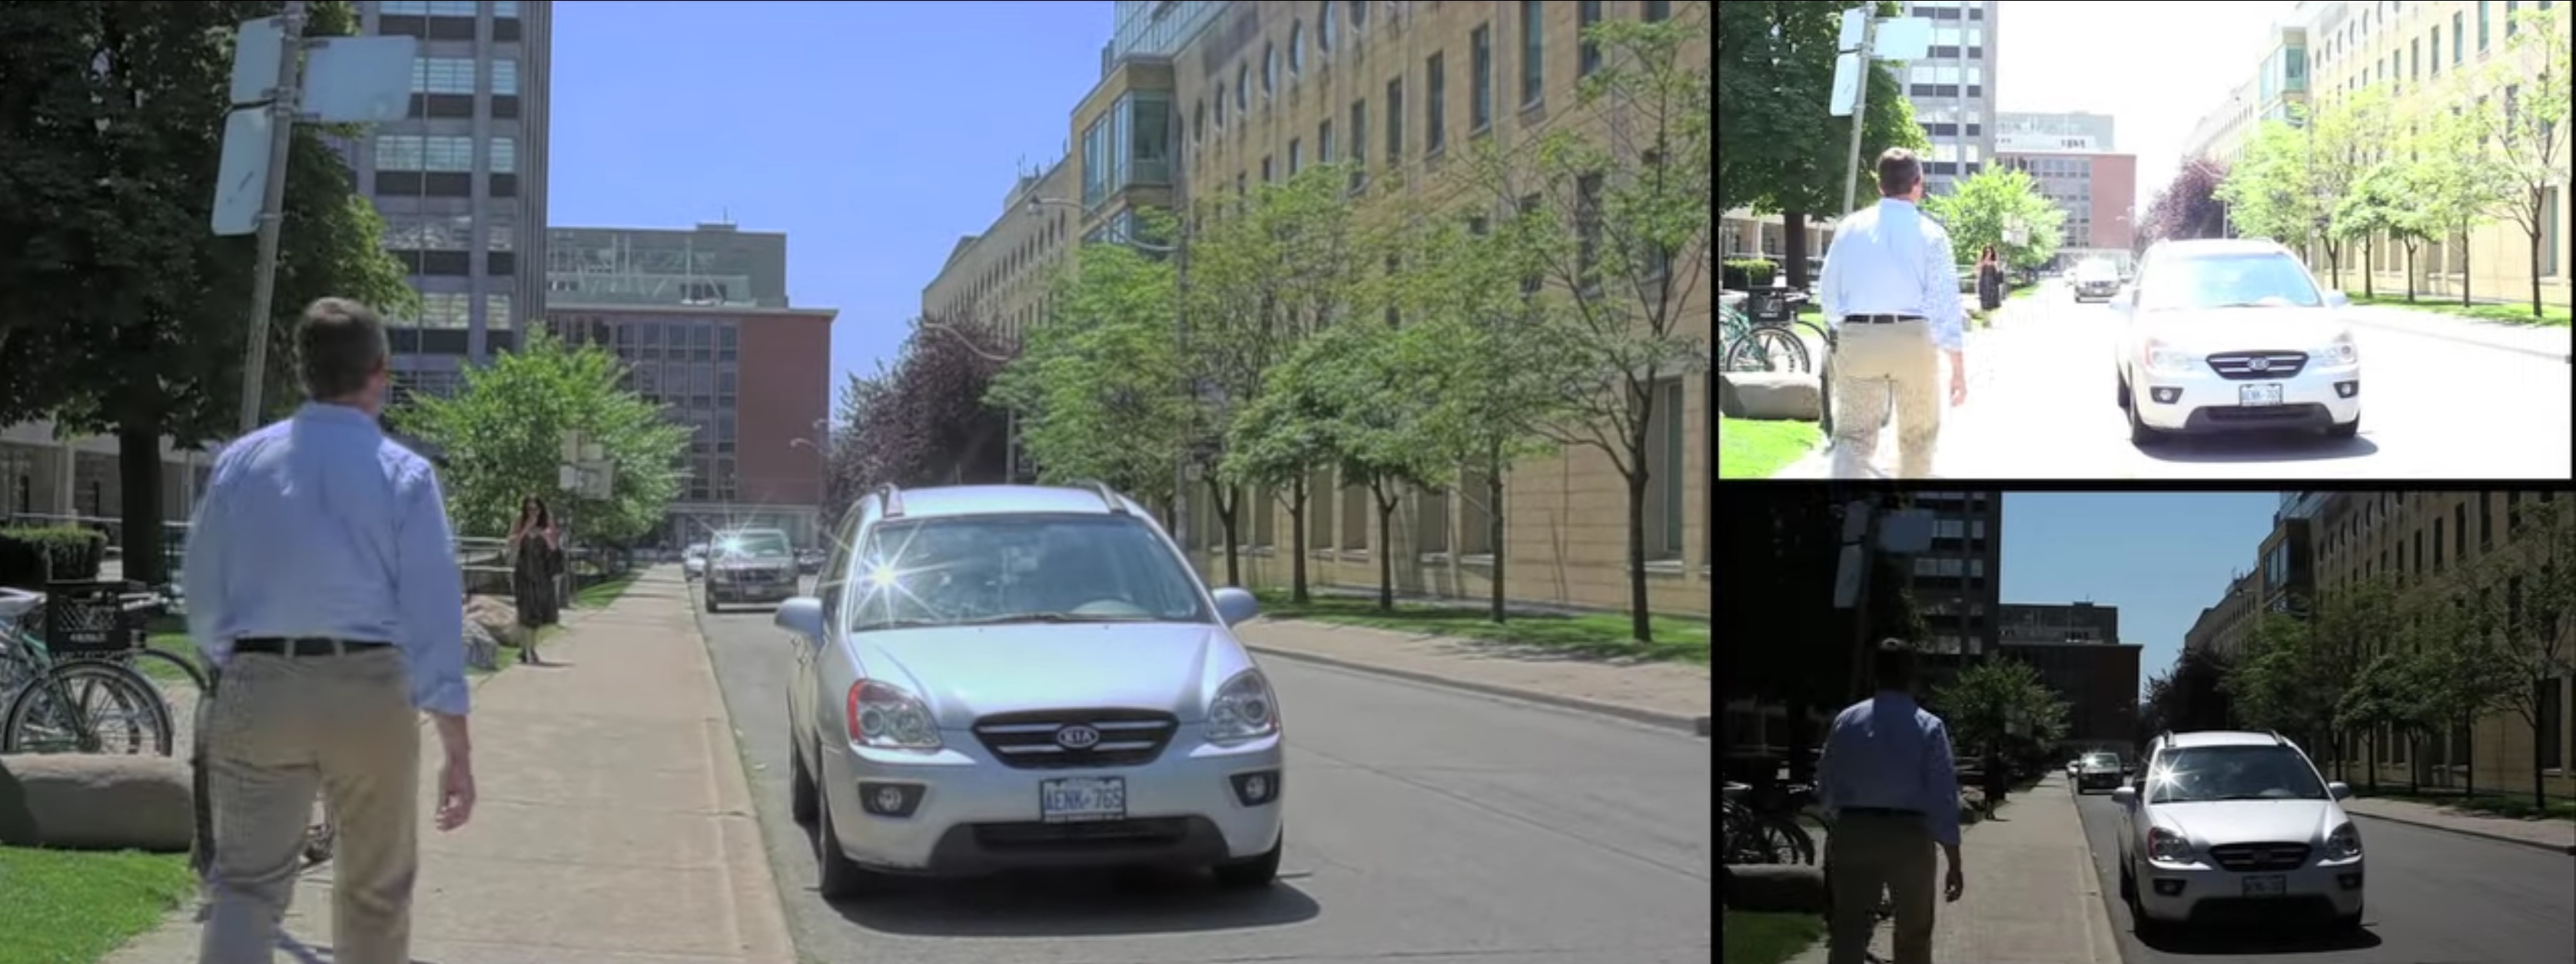
\includegraphics[width=5.5in]{ch2/diagrams/everyday2.jpg}
 \caption{Another example of HDR video captured on the street. At the right side of the frame, the 
final HDR image can see through the car's windshield and have visibility of what's inside the car. The 
additional dynamic range provides better seeing into many situation which often human eye cannot 
see.}
 \label{fig:extremeeveryday2}
\end{figure}

\subsection{Remote Experts and Training}

The Digital Eye Glass can also provide real-time training data and perform real-time tracking. One 
use case is a set of welding instruction is provided to the user in real-time as the person is welding. 
The eyeglasses automatically track and judge the distance and speed required and such real-time 
feedback is critical for the success or failure of the task. In addition, remote experts, who can even be 
oversea, can provide audio and visual feedbacks and perform any corrective actions. 

\begin{figure}
\center
 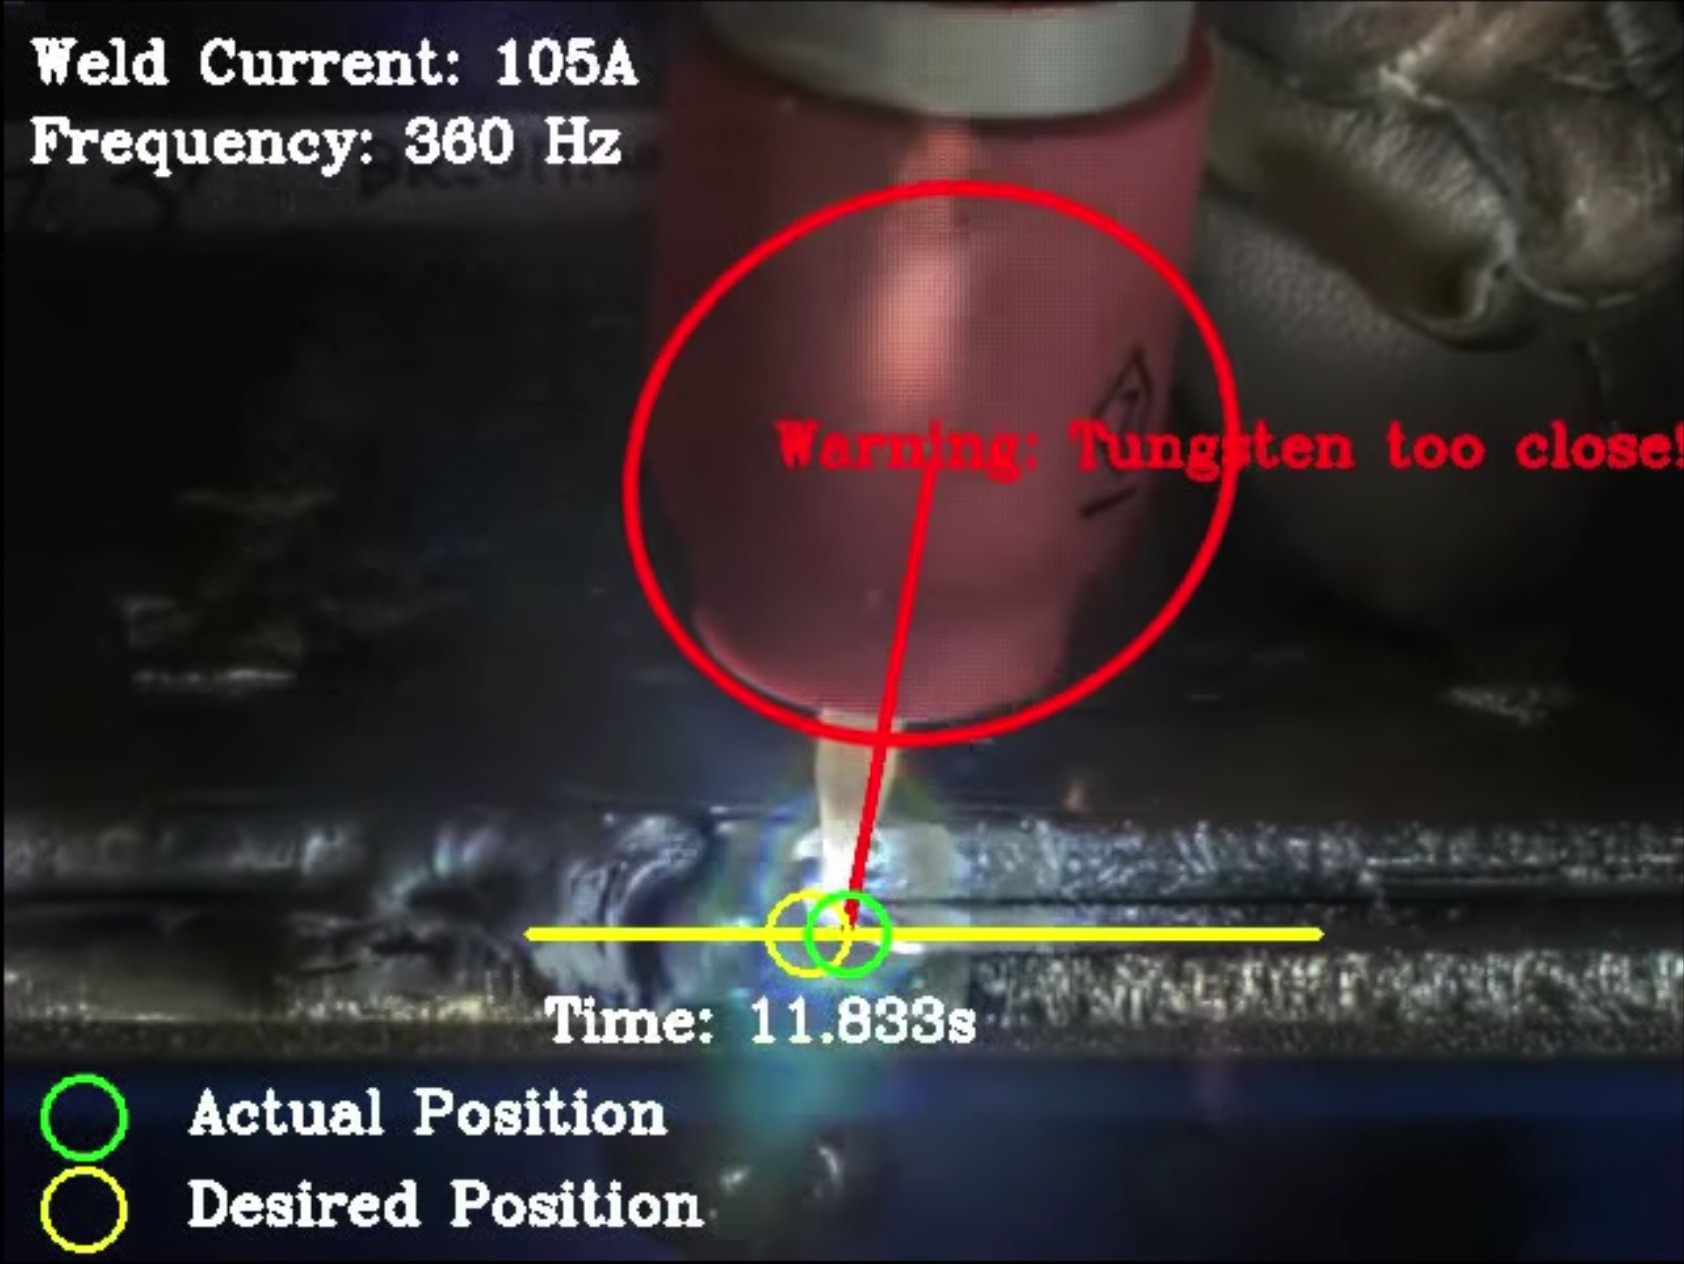
\includegraphics[width=5in]{ch2/diagrams/remote3.jpg}
 \caption{Remote expert application for TIG Welding. An augmented reality interface is overlayed 
onto the actual welding scene to instruct the user on how to weld in real-time. Wearer can see the 
instruction, and get real-time feedback from remote user with the prototype system. Most important, 
the 3D HDR feature allows clear view of the welding works and the instructions all at the same time 
without any distractions.}
 \label{fig:extremeremote}
\end{figure}

One observation is the tracking solution is significantly improved by using the HDR tone mapped 
output. The temporal stability and additional tonal range that is captured by the system have 
significantly improved the robustness of the color-based tracking algorithm. In 
Fig.~\ref{fig:extremeremote}, a continuously adaptive mean shift (CAMShift) algorithm 
\cite{bradski1998real} was implemented to track the TIG welding tool. Even at the extreme condition 
in which the dynamic range of the scene was over million to one with a constantly flicking light 
source, the tracking algorithm can easily adapt to the final HDR scene and tracked the tool from the 
beginning to the end of the video footage. Such improvement can be deployed onto other algorithms 
that relies on image features and create more robust tracking system in the future.

\begin{figure}
\center
 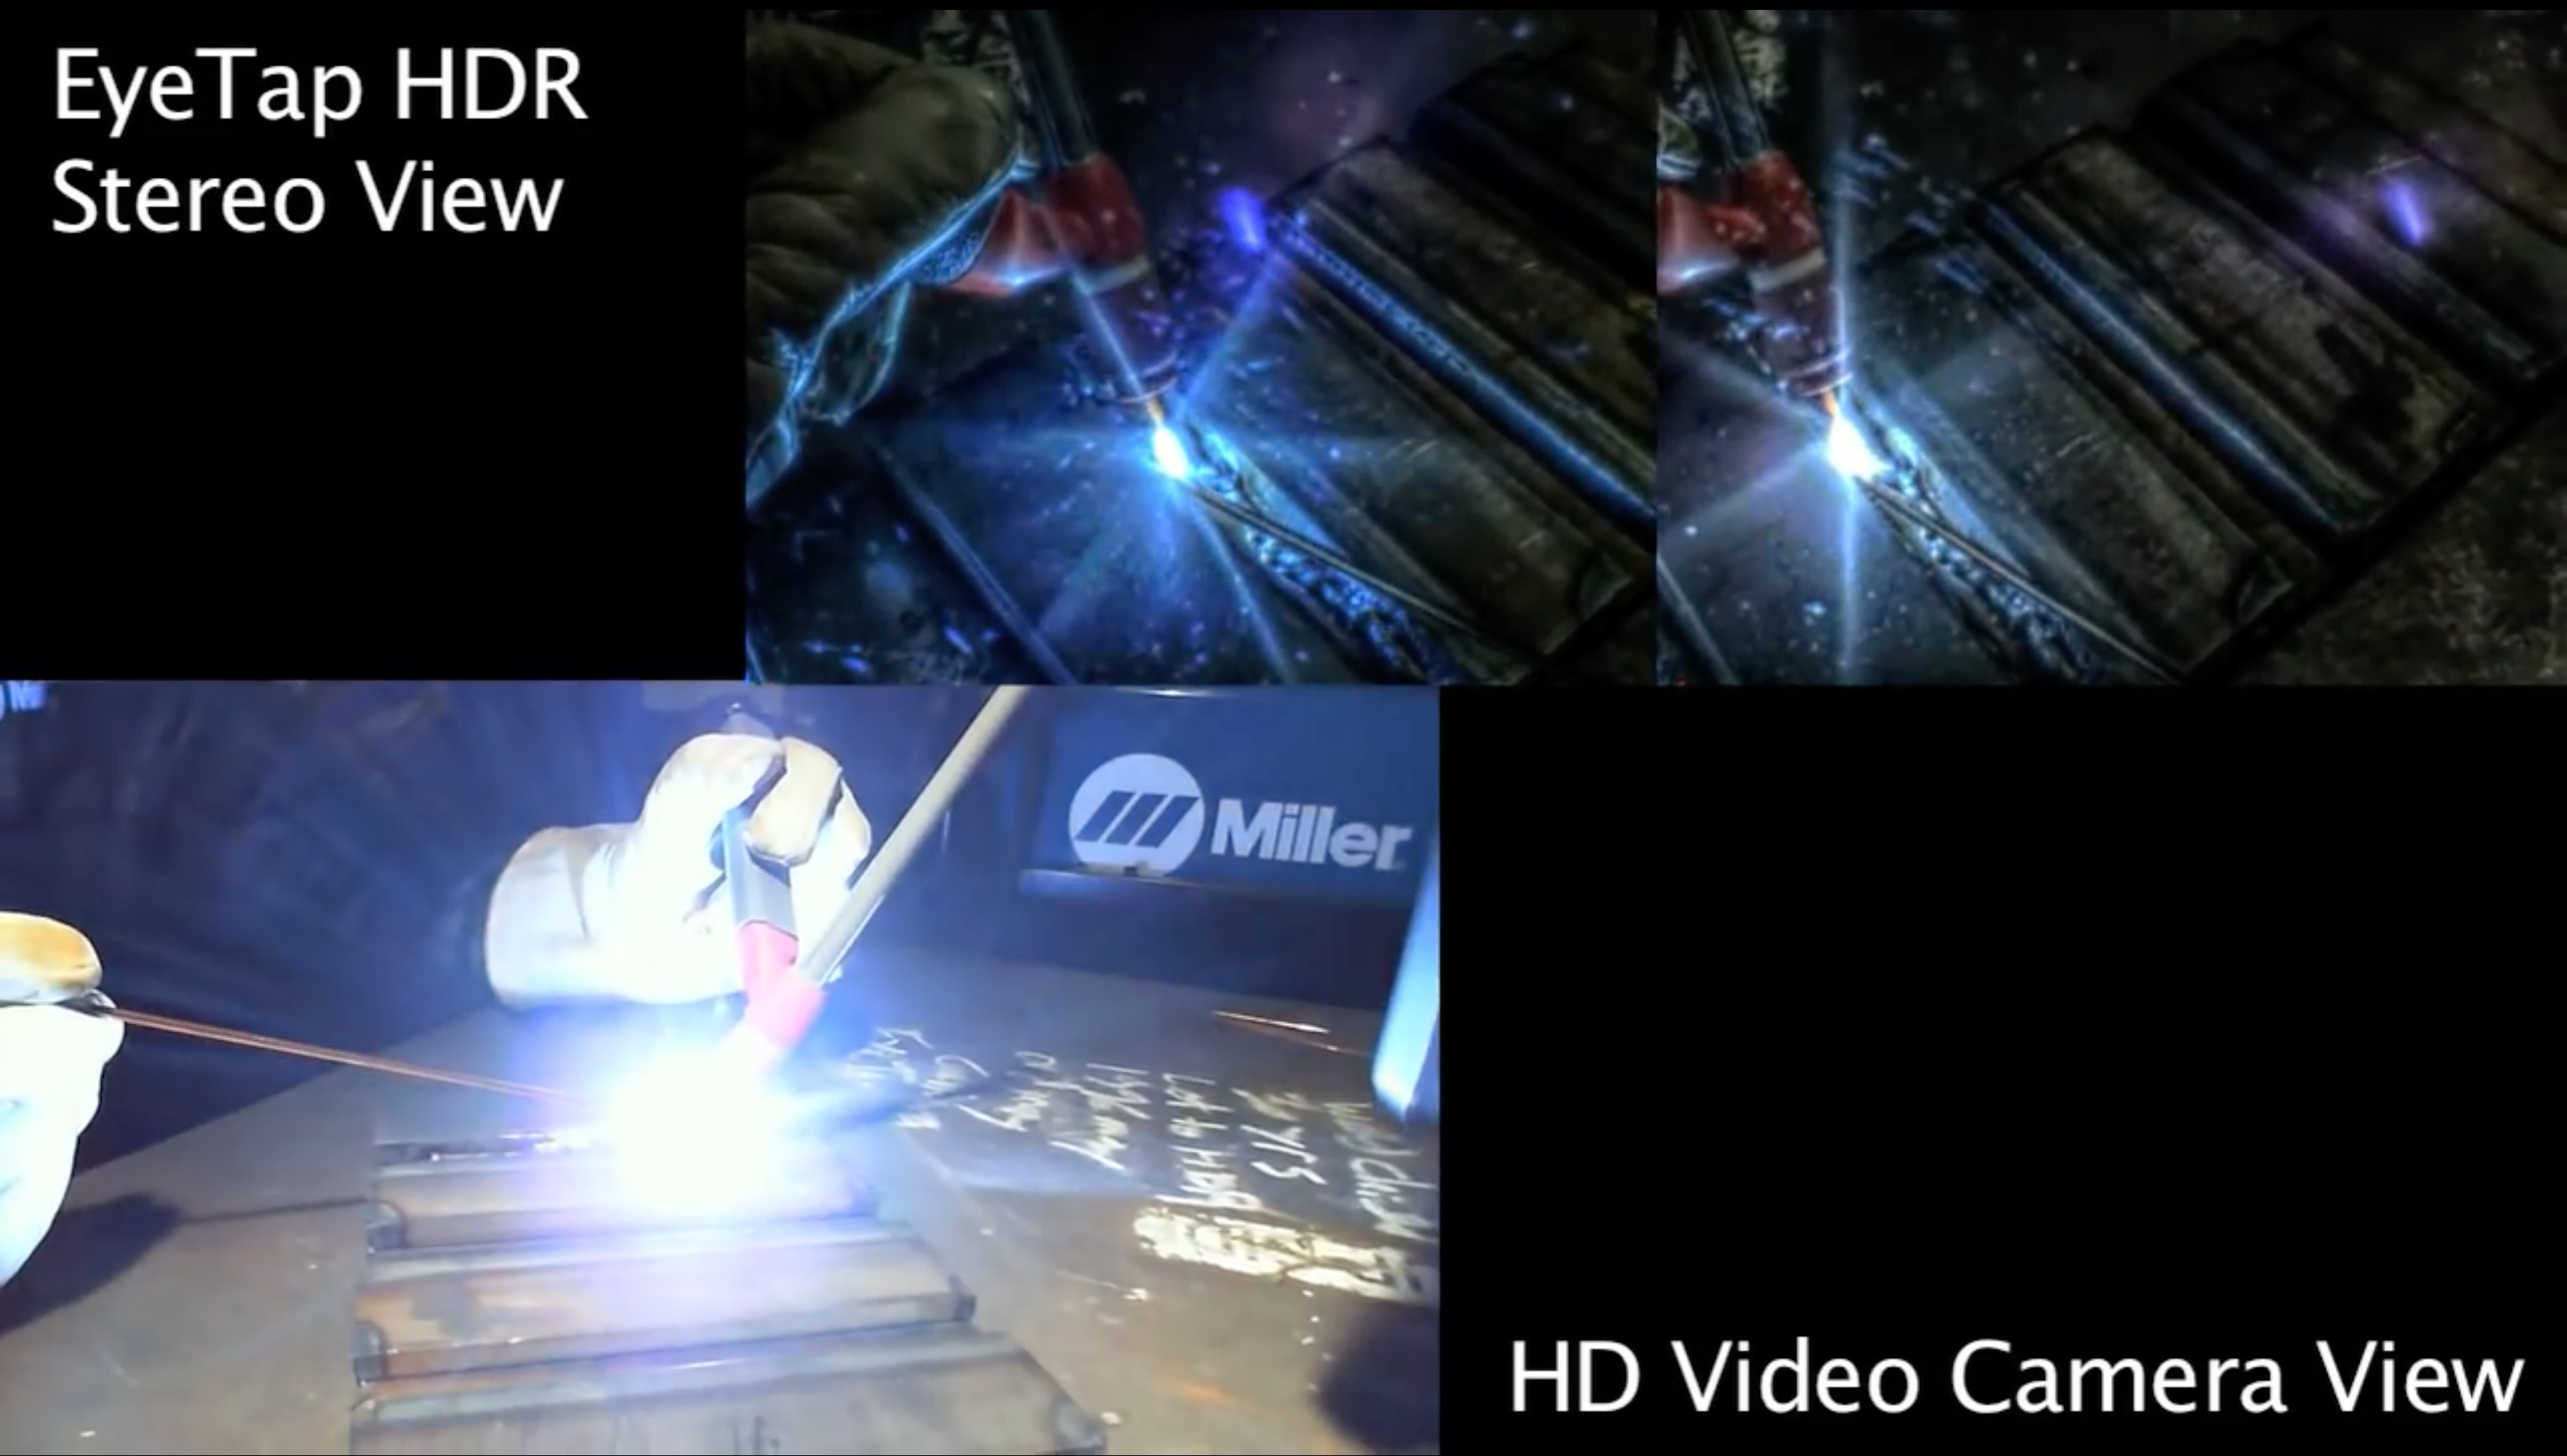
\includegraphics[width=5.5in]{ch2/diagrams/eyetap_3d_view.jpg}
 \caption{3D Stereoscopic View of the final HDR rendering. The bright light from the TIG welding had 
completely `blinded' the sensor in the `` HD Video Camera View'' feed. In comparison, the footage 
shown in the ``EyeTap HDR Stereo View" has much better visibility of the workspace and the 
extremely bright welding job. The left and right images were captured and processed by the 
proposed apparatus and HDR algorithm, and projected back onto each of wearer's eyes in full 
stereo.}
 \label{fig:extreme3dhdr}
\end{figure}


%
%\section{Conclusion and further research}
%We have designed and built a fully functional electric seeing aid that
%uses real-time HDR video processing in a small battery-powered
%device that fits in an EyeTap welding helmet.
%
%Our ultimate goal is to miniaturize the system for use
%in ordinary eyeglasses.  Consistent with that goal will be the installation
%of the Xilinx FPGA (Field Programmable Gate Array) on a circuit board
%shaped as the temple side pieces of ordinary eyeglass frames.
%
%We have proposed a novel computational method using
%LUTs (lookup tables) to compute the HDR (high dynamic range) video in real-time.
%Our system implements a wide variety of different HDR algorithms
%with fixed runtime, regardless of the algorithm selected.
%We demonstrated a speed up of three orders of magnitude for
%non-linear optimization based photo-quantity estimation.

